\documentclass[12pt, french]{report}
\setcounter{secnumdepth}{3}
\setcounter{tocdepth}{1}
\usepackage{graphicx}
\usepackage[T1]{fontenc}
\usepackage[utf8]{inputenc}
\usepackage{lmodern}
\usepackage{amsfonts}
\usepackage{enumitem}
\usepackage[a4paper]{geometry}
\usepackage{babel}
\usepackage{wrapfig}
\usepackage[figurename=Fig.]{caption}
\usepackage{subfig}

\usepackage{longtable} 

\usepackage{makecell}%using for thead

\renewcommand\theadalign{bc}
\renewcommand\theadfont{\bfseries}
\renewcommand\theadgape{\Gape[4pt]}
\renewcommand\cellgape{\Gape[4pt]}

\usepackage[nottoc]{tocbibind}%Automatic approach to add \listoffigures and \listoftables in table of contents

\usepackage{color}   %May be necessary if you want to color links

%Customize chapter format
\usepackage{titlesec, blindtext}
\definecolor{gray75}{gray}{0.75}
\newcommand{\hsp}{\hspace{20pt}}
\titleformat{\chapter}[hang]{\Huge\bfseries}{\thechapter\hsp\textcolor{gray75}{|}\hsp}{0pt}{\Huge\bfseries}
%End customize chapter format


\usepackage{hyperref}
\hypersetup{
    colorlinks=true, %set true if you want colored links
    linktoc=all,     %set to all if you want both sections and subsections linked
    linkcolor=blue,  %choose some color if you want links to stand out
}


\usepackage{quoting,xparse}

\NewDocumentCommand{\bywhom}{m}{% the Bourbaki trick
	{\nobreak\hfill\penalty50\hskip1em\null\nobreak
		\hfill\mbox{\normalfont(#1)}%
		\parfillskip=0pt \finalhyphendemerits=0 \par}%
}

\NewDocumentEnvironment{pquotation}{m}
{\begin{quoting}[
		indentfirst=true,
		leftmargin=\parindent,
		rightmargin=\parindent]\itshape}
	{\bywhom{#1}\end{quoting}}

\usepackage{natbib}

\begin{document}
\renewcommand{\labelitemi}{$\bullet$}
	\begin{titlepage}
		
		\newcommand{\HRule}{\rule{\linewidth}{0.4mm}} % Defines a new command for the horizontal lines, change thickness here
		
		\center % Center everything on the page
		
		%----------------------------------------------------------------------------------------
		%	HEADING SECTIONS
		%----------------------------------------------------------------------------------------
		
		\textsc{\LARGE Université de Montréal}\\[1cm] % Name of your university/college
		\textsc{\Large Faculté des arts et des sciences}\\[0.5cm] % Major heading such as course name
		\textsc{\large Département d’informatique et de recherche opérationnelle (DIRO) }\\[0.3cm] % Minor heading such as course title
		
		%----------------------------------------------------------------------------------------
		%	TITLE SECTION
		%----------------------------------------------------------------------------------------
		
		\HRule \\[0.4cm]
		{ \huge Rapport de stage \\ \bfseries Évaluation du risque de retour à la maison } \\[0.4cm] % Title of your document
		\HRule \\[1.5cm]
		
		%----------------------------------------------------------------------------------------
		%	AUTHOR SECTION
		%----------------------------------------------------------------------------------------
		
		\begin{minipage}{0.4\textwidth}
			\begin{flushleft} \large
				\emph{Auteur:}\\
				Vilon \textsc{Saint-Fleurose} % Your name
				\\MSc, informatique \\Université de Montréal
			\end{flushleft}
		\end{minipage}
		~
		\begin{minipage}{0.4\textwidth}
			\begin{flushright} \large
				\emph{Directeur de recherche:} \\
				Dr. Michalis \textsc{Famelis} % Supervisor's Name
				\\Professeur adjoint \\Université de Montréal
			\end{flushright}
		\end{minipage}\\[1cm]
			~
			\begin{minipage}{0.4\textwidth}
				\begin{center} \large
					\emph{Superviseur:} \\
					 Nicolas \textsc{Coallier} % Supervisor's Name
					\\Vice-Président Exécutif, TIC \\ML+
				\end{center}
			\end{minipage}\\[1cm]
		
		% If you don't want a supervisor, uncomment the two lines below and remove the section above
		%\Large \emph{Author:}\\
		%John \textsc{Smith}\\[3cm] % Your name
		
		%----------------------------------------------------------------------------------------
		%	DATE SECTION
		%----------------------------------------------------------------------------------------
		
		{\large \today}\\[1cm] % Date, change the \today to a set date if you want to be precise
		
		%----------------------------------------------------------------------------------------
		%	LOGO SECTION
		%----------------------------------------------------------------------------------------
		
		
\includegraphics[width=3cm, height=1cm]{images/logo.png} % Include a department/university logo - this will require the graphicx package
		
		%----------------------------------------------------------------------------------------
		
		\vfill % Fill the rest of the page with whitespace
		
	\end{titlepage}
		
\tableofcontents
\newpage	
\addcontentsline{toc}{chapter}{Remerciements}
\chapter*{Remerciements}
Je veux commencer d'abord par remercier le Grand Dieu Tout-Puissant, le Créateur de l'univers, des cieux et de la terre qui m'a donné la vie, la santé, les opportunités et tout ce dont j'avais besoin pour faire cette grande et belle étude à l'université de Montréal. Il a rendu toutes choses possibles en ma faveur, moi qui suis pécheur et désobéissant; immérité de toutes ces grâces. Il m'accompagnait toujours dans les moments les plus difficiles de ma vie, Il ne m'a jamais laissé seul; surtout dans les moments où je devais payer les frais de scolarité qui étaient si énormes et impossibles à payer de mon propre compte. A un Dieu si merveilleux et si bon, je Lui dois beaucoup de reconnaissance.  \\
	
	Je remercie aussi ma femme qui m'a beaucoup supporté pendant plus de deux années d'études. Elle n'a jamais murmuré, ni découragé quand nous devions passer par des moments difficiles de notre vie conjugale à cause de ces études. Elle a mis toutes ses ressources disponibles pour entretenir la famille et payer mes études quand j’étais moi-même dans l’impossibilité de travailler. Vraiment, ma femme est une bénédiction dans ma vie, un cadeau venant de Dieu. Je t’aime ma chérie. \\
	
	Je tiens à remercier le professeur Michalis Famelis d’avoir accepté être mon directeur de recherche et supervisé ce stage, il est toujours là pour m’encourager et me pousser vers l’avant. Il répond toujours présent à tous mes appels, il est toujours disponible pour me rencontrer, me parler et me conseiller ; même en dehors du cadre universitaire.  \\
	
	Je remercie Nicolas Coallier et toute l’équipe ML+ qui ont accepté que je sois leur stagiaire, ils ont placé  leur confiance en moi quoiqu’ils ne me connaissaient pas encore. Cette équipe, quoique jeune, est très dynamique et chaleureuse, c’est une équipe motivante qui stimule la connaissance. J’ai dû apprendre beaucoup de choses par rapport à eux.
	Finalement, je présente mes sincères remerciements à toute la communauté universitaire, à DIRO en particulier. Merci pour la formation prestigieuse que vous m’avez fournie. Cette formation est si solide qu’elle m’aidera rapidement à intégrer le marché du travail sans perdre de temps. 
	
\newpage

\chapter*{Préface}
Nous développons ce rapport en vue d'achever notre étude de maîtrise en informatique faite à l'université de Montréal. Nous avons inscrit notre maîtrise avec option stage, ce qui exige la redaction d'un rapport au terme de ces études. Nous avons, d'abord réalisé le stage à l'entreprise ML+ située à l'adresse suivante: 338, rue St-Antoine est, Montréal. C'est une jeune entreprise dynamique et spécialisée en science de données. Elle développe des outils pour aider les entreprises à prendre leurs décisions stratégiques tout se basant sur des données historiques des entreprises. \\

C'est une expérience enrichissante d'avoir eu l'opportunité de faire ce stage dans cette entreprise, j'ai pu apprendre beaucoup de choses tant sur machine learning que sur les sciences de données en général. Ces connaissances acquises m'ont ouvert  la porte pour pouvoir rédiger ce rapport. Ce dernier permet d'évaluer le risque d'un patient de retourner chez lui après une opération contre l'arthrose (douleur ressentie au niveau des os).  

\newpage

\listoffigures

\newpage

\listoftables

\newpage

\addcontentsline{toc}{chapter}{Résumé}
\chapter*{Résumé}
L'arthroplastie totale de la hanche et du genou permet à diminuer considérablement la douleur
et améliore la fonction chez les personnes atteintes d'arthrose avancée. Selon une étude publiée en 2012 dans le journal ISRN Orthopedics, les auteurs Bronislava Bashinskaya et al. \cite{key2} ont constaté que : \guillemotleft Le
vieillissement de la génération du "baby boom", combiné au désir de
maintenir un mode de vie actif et sans douleur, entraînera une augmentation
du nombre annuel de chirurgies de remplacement articulaire pratiquées dans
États Unis\guillemotright. Dans un rapport publié en Avril 2007 par les orthopédistes Steven M Kurtz, Kevin Ong, Edmund Lau et Michael T Halpern \cite{key3}, membres de l'Académie américaine des chirurgiens orthopédiques, ils ont prédit que : \guillemotleft  
D'ici 2030, la demande d'arthroplasties totales de la hanche totale devrait augmenter de 174\% pour atteindre 572 000. La demande pour les arthroplasties totales du genou primaire devrait augmenter de 673\% à 3,48 millions de procédures
 \guillemotright.
Face à l'augmentation continue du nombre de chirurgies de remplacement, il devient crucial aux administrateurs des hôpitaux de déterminer si les patients doivent rester à l'hôpital pour une réadaptation après leur 	chirurgie ou s'ils doivent être renvoyés à la maison puisque les coûts associés à une réadaptation doivent être pris en charge par les hôpitaux. Il est important de souligner que la majorité des compagnies d'assurance santé aux États Unis n'assument pas les coûts liés à la réadaptation des patients. Ces frais qui sont très élevés (entre 15,000 à 30,000 \$ par patient) doivent être assurés par les hôpitaux. Pour prendre la décision de retour ou non, les chirurgiens tiennent compte des antécédents médicaux du patient et l'état de santé du patient après l'arthroplastie, ce qui est un travail difficile à effectuer manuellement puisque le nombre de patients dans une base de données orthopédiques sont très nombreux. Dans notre projet de stage, nous avons développé un modèle de machine learning (ML) qui aide à prendre cette décision de façon automatique. Nous avons aussi construit un web API qui fait la connexion avec le modèle, ce qui est utile pour les orthopédistes qui n'ont pas de connaissances en ML. On a conçu un interface utilisateur qui rend notre système convivial et facile à utiliser. 
   	
\newpage
\chapter{Introduction générale}	
\section{Contexte}
Le système de santé américain est contrôlé en majeure partie par des compagnies privées, le gouvernement américain ne finance qu'une partie minoritaire de la population. Ce système  repose sur deux sources de financement. D'abord on a le financement public géré par le programme fédéral Medicare qui vise seulement les personnes âgées de plus de 65 ans et celles qui sont gravement handicapées. D'après Europusa \cite{key4}, une compagnie européenne spécialisée dans l'accompagnement des européens qui veulent immigrer aux états-unis : \guillemotleft Cette source de financement couvre 26\% de la population américaine dont 15 \% sont des personnes agées et handicapées et 11\% sont des familles pauvres avec enfants.  \guillemotright. La deuxième source de financement qui est un financement privé touche tout le reste de la population soit 74\%. L’assurance est donc majoritairement privée aux Etats-Unis. Les Américains sont assurés en général via leurs employeurs ou sinon de manière individuelle lorsque leur employeur ne propose pas d’assurance ou qu’ils travaillent comme travailleurs autonomes. La composante « 	assurance médicale » dans le choix d’un emploi est donc un critère important. En général le système de santé américain est échoué parce qu'une grande partie de la population se retrouve sans assurance santé. C'est un système libéral fondé sur le principe du marché et de la concurrence qui s’organise autour d’assurances privées souvent liées à l’emploi et d’une assurance maladie obligatoire. \\

Les compagnies d'assurance santé américaines ne couvrent pas les coûts associés à une réadaptation d'un patient après une arthroplastie (Opération ayant pour but de rétablir la forme et la mobilité d'une articulation abîmée ou bloquée.). Il revient à l'hôpital de couvrir ces coûts qui sont très élevés. Selon le docteur orthopédiste Jonah Hebert-Davies qui a fait ses études de spécialité en Orthopédie à l'université de Seattle, Washington aux États-Unis \footnote{Pour informations sur la bibliographie du docteur, consultez http://www.orthop.washington.edu/?q=faculty-profiles/jonah-hebert-davies-md-frcsc.html}, les coûts estimés sont entre 15,000 \$ à 30,000 \$ par patient. Ce qui revient à une grande perte financière pour les hôpitaux.  La décision de maintenir ou de renvoyer un patient après une arthroplastie devient une question préoccupante dans la mesure où elle pourrait réduire le coût budgétaire des hôpitaux. Si la décision prise est de renvoyer le patient, l'hôpital est le gagnant sinon il est le perdant. \\ 

D'autres part, l'arthrose (maladie qui touche les articulations et caractérisée par la douleur et la difficulté à effectuer des mouvements articulaires \cite{key12}) touche environ 27 millions d'adultes aux États-Unis \cite{key11}.  Ce qui augmente considérablement le nombre d'arthroplastie dans les hôpitaux, et aussi le poids de travail des médecins à savoir quand est-ce qu'il ya une réadaptation ou non.\\

Il est un travail fastidieux pour les spécialistes orthopédistes de vérifier manuellement les données médicales d'un patient pour pouvoir décider s'il doit être renvoyé ou non. Ce travail consiste en ce que les données médicales d'un dossier patient sont très volumineuses. Seulement pour déterminer les conditions médicales antécédentes du patient, quarante six (46) colonnes pré-opératoires (C'est-à-dire les conditions de santé du patient avant une opération arthroplastie) doivent être prises en compte. Pour calculer les conditions médicales, le médecin orthopédiste doit additionner toutes les valeurs des colonnes pré-opératoires après avoir substitué ces valeurs soit par un(1), soit par deux(2) ou par trois(3) comme expliqué à la section de feature engineering. En plus de calculer les conditions médicales, il y a d'autres calculs à faire comme déterminer le niveau diagnostique du patient en se basant sur  les trois niveaux diagnostiques existant dans l'ensemble de données. Toutes ces démarches sont expliquées en détail dans la section de feature engineering. \\

Considérant le nombre grandissant d'arthroplastie dans les hôpitaux américains et tous les travaux manuels qu'un orthopédiste doit réaliser avant de décider le retour ou non d'un patient à la maison, nous estimons que créer un outil pour automatiser cette tâche est un projet pertinent. Le but de notre stage consiste à développer cet outil-là qui aidera les orthopédistes américains à prendre cette décision de façon automatique et sans perdre de temps.  \\

\section{Ingénierie des exigences}

Nous supposons qu'il existe déjà un jeu de données disponibles contenant toutes les informations touchant un grand nombre de patients et que chaque échantillon de ce jeu de données est un dossier patient. Nous supposons aussi que ce jeu de données possède des caractéristiques suffisantes pour décider si un patient doit être renvoyé ou non. Nous considérons aussi que ce jeu de données est composé de patients qui font l'objet d'une décision de retour. Si toutes ces conditions sont réunies, nous pouvons profiter des différentes technologies de la science de données, du marching learning et l'ingénierie de logiciels pour développer un outil d'aide à la décision qui aide les orthopédistes à prendre la décision de retour automatiquement. \\

Les technologies de la science de données sont conçues pour développer des outils qui permettent de prendre des décisions à partir d'un ensemble de données existantes. Le machine learning qui est un sous-ensemble de la science de données permet de modéliser à partir du même ensemble de données. Dans le chapitre 2, nous expliquons le cycle de vie du travail du data scientist en détail. Ce que nous proposons comme solution dans notre projet. Nous avons réalisé ce cycle complet pour implémenter notre système d'aide à la décision. \\

Il y a deux grandes phases impliquées dans le processus de développement de notre projet. La première phase est la construction d'un modèle machine learning et la deuxième est le déploiement du modèle construit, cette phase consiste en la création d'un API nommé Ortho, c'est une phase d'ingénierie de logiciels. Pour les deux phases, nous avons crée deux diagrammes, un diagramme de cas d'utilisation qui donne une vision globale du comportement fonctionnel de notre notre système et un diagramme d'états qui explique le processus du développement du modèle. Nous donnons une brève explication de chaque diagramme et leurs différents composants. \\

Nous commençons d'abord par le diagramme de cas d'utilisation. Il consiste en la phase de déploiement du modèle. Ce diagramme explique comment les orthopédistes peuvent utiliser notre système. la figure \ref{usecase} représente une vue de notre diagramme, chaque cas représente une unité discrète d'interaction entre un utilisateur (Orthopédiste ou administrateur) et notre système. Voici une brève explication des acteurs et de chaque cas:
\begin{enumerate}
	\item \textbf{Actors.} Les acteurs sont des orthopédistes et les administrateurs du système qui sont des orthopédistes ayant des droits et privilèges d'évaluer, de suivre et de gérer le modèle déployé;
	\item \textbf{Predict.} Les orthopédistes peuvent utiliser cette section en vue de prédire si les patients doivent rester à l'hôpital ou retourner chez eux. Pour accomplir cette tâche, il est obligatoire de remplir un formulaire.
	\item \textbf{Fill form.} Pour prédire, il faut remplir le formulaire qui contient les informations du dossier médical du patient. On recueille les informations pertinentes pour la prise de décision telles que les conditions médicales, les diagnostiques antérieures, l'indice de masse corporelle (BMI en anglais) etc. 
	\item \textbf{Evaluate.} Permet d'évaluer le modèle sur de nouvelles données prédites. On peut comparer l'évaluation faite au moment de la construction du modèle et celle faite au moment de la prédiction. L'évaluation exige une authentification.  
	\item \textbf{Monitor.} Permet de suivre périodiquement le modèle pour déterminer si les performances s'améliorent ou si elles détériorent. Exige une authentification.
	\item \textbf{Manage.} Permet d'optimiser le modèle sur de nouvelles données en essayant d'utiliser de nouveaux hyper-paramètres en vue de comparer les résultats. Exige une authentification.
	\item \textbf{Authenticate.} Permet l'authentification du système. Exige un nom utilisateur et un mot de passe.
\end{enumerate}

\begin{figure}[h]
	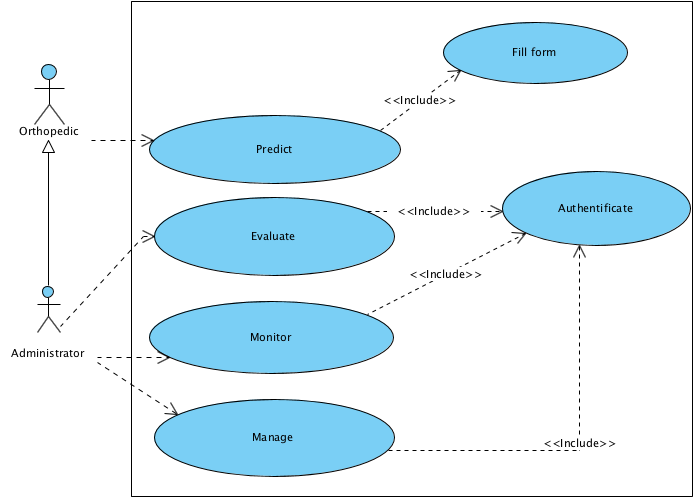
\includegraphics[width=17cm, height =9cm]{images/UseCaseDiag.png}
	\caption{A use-case diagram for describing our API Ortho}
	\label{usecase}
\end{figure}  

Nous poursuivons avec le diagramme d'états présenté dans la figure \ref{MLUseCase}.  Il décrit les différents états qui constituent le développement de notre modèle ML. Voici un bref résumé de ce fait chaque état: 

\begin{enumerate}
\item \textbf{API Ortho.} L'API fait la connexion entre le système du machine learning et le système du déploiement. Il accède au modèle qui a été sérialisé. 
\item \textbf{Gather.} Permet de récupérer les données du dataset;
\item \textbf{Clean.} Permet de nettoyer les données en imputant les données nulles et en supprimant les variables que ne sont pas pertinentes;
\item \textbf{Explore.} Permet d'explorer les données pour voir les différentes corrélations qui existent entre les variables et l'étiquette;
\item \textbf{Transform.} Création de nouvelles variables en fonction de celles qui existent déjà dans l'ensemble des données. 
\item \textbf{Preprocess.} Un pré-traitement des données avant de les envoyer à l'algorithme de machine learning. Par exemple, les algorithmes de machine learning ne traitent pas les textes, il faut les convertir en valeurs numériques avant de les envoyer aux algorithmes. 
\item \textbf{Train.} C'est la phase d'entrainement de modèles pour déterminer lequel est meilleur pour notre ensemble de données.
\item \textbf{Serialize.} Sauvegarde le meilleur modèle pour son utilisation future. 
\end{enumerate}


\begin{figure}[h]
	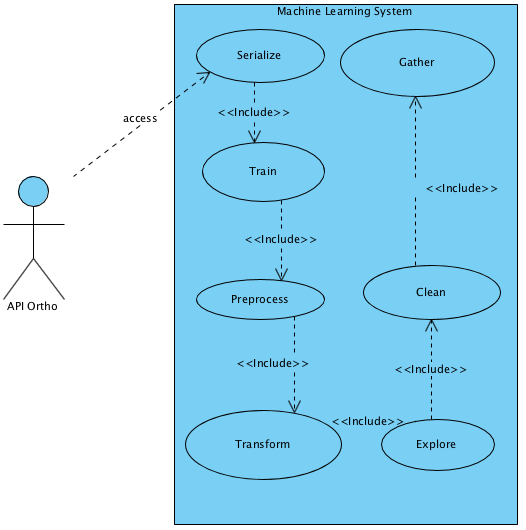
\includegraphics[width=13cm, height =13cm]{images/APIML.png}
	\caption{A use-case diagram for describing our Machine Learning System}
	\label{MLUseCase}
\end{figure} 

La suite de ce rapport est composé de plusieurs chapitres et chaque chapitre a des sections, subsections etc. Le chapitre 2 donne un contexte théorique des différents éléments qui sont importants pour notre projet. Le chapitre 3 décrit en détail la construction de notre modèle machine learning. Le chapitre 4 décrit la création de l'outil Ortho qui fait la connexion avec le modèle machine learning. Le chapitre 5 montre comment nous évaluons les différents évaluations morceaux de notre système. Le chapitre 6 détaille les travaux connexes liés au développement d'API machine learning, la technique de re-échantillonnage, aux algorithmes ensemblistes etc. Le chapitre 7 fait la conclusion de notre projet.


\newpage

\chapter{Contexte théorique}
\section{Introduction}

Tout projet informatique suppose qu'on doit délivrer un produit fini et utilisable accomplissant un certain nombre d'objectifs. Il y a toujours une équipe qui travaille durement pour réaliser ou implémenter ces genres de projets. Tout développement informatique passe nécessairement par la pratique ce qui exige souvent l'application de beaucoup de concepts étudiés en théorie. Dans tout rapport portant sur la réalisation d'un projet scientifique et technique, il s'avère utile et important d'établir un contexte théorique dans le but de faire ressortir les différents cadres théoriques. Nous allons, dans ce chapitre, présenter quelques concepts théoriques importants abordés dans le cadre de notre projet.\\

Généralement, nous nous mettons l'accent sur un sous-ensemble de tous les concepts jugés pertinents pour la réalisation de notre projet. Par exemple, le machine learning est un champ de recherche informatique de plusieurs décennies de travaux de recherche, il est impossible de d'aborder dans un seul chapitre tout ce qui a trait au ML, par contre nous nous concentrons sur les éléments les plus essentiels pour notre projet. \\      

La suite de ce chapitre se subdivise comme suit : la deuxième section est une approche globale sur les sciences de données. Nous estimons que c'est important parce qu'aucun modèle de machine learning ne peut être construit sans d'abord réaliser une phase d'exploration de données; or les sciences de données peuvent être définies comme étant une combinaison entre l'exploration de données et la modélisation de données. La troisième section se porte sur le machine learning qui est le cœur même de notre projet; comme on avait précisé au paragraphe antérieur, nous considérons seulement un sous-ensemble de concepts jugés utiles pour notre projet. La quatrième traite du problème de classification en ML; puisque notre projet était un problème de classification, nous décidons de le consacrer une section indépendante. La cinquième et dernière se porte sur les classes déséquilibrées car notre ensemble de données était déséquilibrée.     

\section{Sciences des données}

On ne peut pas parler de machine learning sans avoir parlé des sciences de données. Car la modélisation des données est une étape des sciences de données, quoique la plus importante. Les sciences de données nous permettent de prendre un ensemble de données brutes, les explorer et les modéliser dans le but d'extraire des connaissances utiles à la prise d'une décision. Comme son nom l'indique, la science des données n'est possible que lorsqu'on dispose d'un jeu de données qu'on appelle données historiques. Ces dernières sont des données recueillies à partir de la collecte d'informations. Les données peuvent être sous diverses formes, structurées ou non. D'une façon générale, pour traiter un problème en sciences de données, trois conditions sont nécessaires : (1) il faut avoir les données disponibles dans un format adéquat; (2) définir des objectifs précis de ce qu'on veut faire avec les données; (3) et savoir comment est-ce qu'on va procéder pour réaliser ces objectifs. \\

Les sciences de données peuvent être considérées comme une jonction entre l'informatique et les statistiques. Du coté de l'informatique, c'est la modélisation de données et tandis que du coté des statistiques, c'est l'exploration des données. Nous définissons la modélisation comme étant l'utilisation d'un algorithme d'apprentissage sur un ensemble de données bien préparé; on entend par \textit{bien préparé}, quand un jeu de données ne contient pas des données nulles, vides et textuelles.  Quant à l'exploration,  c'est la phase de visualisation et de préparation des données brutes qui peuvent être sous diverses formes. \\

Les sciences de données offrent des méthodes automatisées pour l'analyse prédictive d'un ensemble de données généralement massif. Le but est d'apporter des solutions à des problèmes spécifiques. Au début de l'ère de de l'intelligence artificielle, l'analyse des données massives était compliquée parce que la capacité de calcul des ordinateurs était faible. Avec l'augmentation exponentielle des capacités de ordinateurs, l'explosion quantitative des données numériques devient de moins en moins un problème. Il faut noter qu'en Machine Learning, plus on a de données, plus l'analyse prédictive est fiable. Les algorithmes d'apprentissage fonctionnent mieux avec de grandes quantités de données. Quand le jeu de données est volumineux, on peut faire facilement la validation croisée qui est une technique par laquelle on subdivise aléatoirement un ensemble de données en plusieurs parties dans le but d'obtenir un meilleur apprentissage. La grande quantité de données permet aussi un séparation de données adéquate entre l'ensemble d'entrainement et l'ensemble de test.\\  

Grâce à la croissance de la capacité de stockage des ordinateurs, l'apparition des algorithmes d'apprentissage puissants et la puissance de calcul des ordinateurs, la profession de \textit{scientifique de données} a vu le jour. Yannis Chaouche \footnote{https://openclassrooms.com/courses/initiez-vous-au-machine-learning/comment-resoudre-un-probleme-de-data-science}, professeur et expert en machine learning, a publié sur le site web OpenClassrooms, un cours intitulé  \guillemotleft \textit{Initiez-vous au machine learning}\guillemotright  où il a défini le cycle de travail d'un scientifique de données. D'après lui ce cycle comprend:

\begin{pquotation}{Professeur Yannis Chaouche}
		\noindent 1. la récupération des données utiles à l'étude;\\
		2. le nettoyage des données pour les rendre exploitables;\\
		3. une longue phase d'exploration des données afin de comprendre en profondeur l'articulation des données;\\
		4. la modélisation des données;\\
		5. l'évaluation et interprétation des résultats;\\
		6. la conclusion de l'étude : prise de décision ou déploiement en production du modèle.
\end{pquotation}  
		

La figure \cite{key6}, implémentée par le professeur Yannis,  nous donne une vue générale du travail d'un scientifique de données. Cette figure est une façon de schématiser les différentes étapes qu'on a définies précédemment. Comme stagiaire en science de données, nous avons suivi minutieusement, dans le cadre de notre projet, le cycle de travail complet défini par le professeur Yannis. Depuis la récupération des données jusqu'au déploiement d'un système en production. Nous expliquerons en détail dans les deux prochains chapitres comment nous implémentons ce cycle au sein de notre projet. \\ \\
\begin{figure}[h]
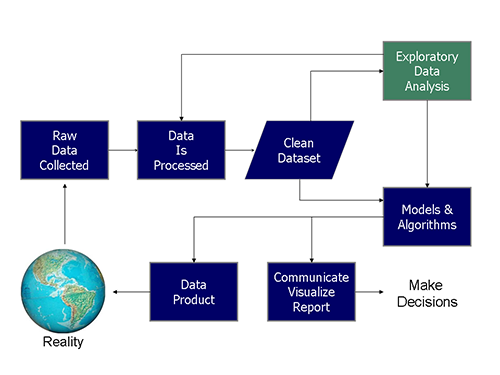
\includegraphics[]{images/workflow_datascientis.png}
\caption{Cycle de travail d'un scientifique de données}
\label{workflow_datascientis}
\end{figure}

\subsection{Données.}

Comme nous avons précédemment dit, les données sont éminentes pour un travail de scientifique de données. S'il n'y a pas de données ou si elles ne sont pas disponibles, on ne peut rien faire. Dans les organisations les données n'ont pas les mêmes niveaux d'importance, par exemple les données juridiques sont de haute confidentialité, personne ne peut avoir accès à moins que les concernés donnent une autorisation légale. Il est toujours difficile d'obtenir les données parce que cela peut compromettre une institution; souvent il faut signer un contrat de confidentialité qui prévoit une sanction sévère s'il y a une violation.  Les données constituent la ressource principale pour qu'un scientifique de données puisse effectuer son travail correctement. 

\subsubsection{Types de données} 
Les données, de part leurs natures, peuvent être quantitatives ou qualitatives. Pour mieux explorer un ensemble de données, il faut savoir distinguer le type de chaque donnée. Quand on parle de type de données ici, il ne faut pas confondre avec type de données qu'on a l'habitude d'utiliser en programmation informatique dans les langages à typage dynamique; mais il faut les considérer d'un point de vue ML. 

\paragraph{Données quantitatives.} Les données quantitatives sont des données qu'on peut mesurer ou qui peuvent prendre une valeur quelconque, avec lesquelles on peut faire des calculs numériques tels que la moyenne, l'addition, la multiplication, la division entre autres. Ces types de données permettent de répondre à la question du type \guillemotleft combien \guillemotright. Par exemple combien de patients y-a-t-il dans la base de données? La réponse pourrait être 3200 qui est une donnée quantitative. Il existe deux catégories de données quantitatives : données quantitatives continues et données quantitatives discrètes. Les premières peuvent n'importe qu'elle valeur dans un ensemble de valeurs, par exemple la température, les PIB,le taux de chômage etc. Les deuxièmes ne prennent qu'un nombre limité de valeur dans un ensemble de valeur, par exemple le nombre d'enfants dans une famille, le nombre de chambres dans un appartement etc. 
    
\paragraph{Données qualitatives.} 
Les données qualitatives décrivent les qualités ou les caractéristiques. On ne peut pas les compter ni faire de calcul avec ces données, on peut les comparer ou éventuellement les trier. Les valeurs qualitatives ne peuvent pas être des nombres, sinon un ensemble de modalités; elles permettent de répondre à la question de la forme \guillemotleft Quel type \guillemotright ou \guillemotleft Quelle catégorie \guillemotright. On distingue aussi deux catégories de données qualitatives : données qualitatives nominales (ou catégorielles) et données qualitatives ordinales. Les premières catégories sont celles dont les modalités ne peuvent ordonnées, par exemple la couleur des yeux, le sexe, la région d'appartenance etc. Les deuxièmes catégories peuvent être ordonnées selon un ordre logique, par exemple les tailles des vêtements, le degré d'accord à un test d'opinion (fortement d'accord, d'accord, pas d'accord ou fortement pas d'accord).

\subsection{Problématique.}
Tout projet de science de données suppose la résolution d'un problème, ce genres de projets commencent toujours par le constat d'un problème. Il faut qu'on soit en mesure de définir clairement ce qu'on veut résoudre et comment on va le résoudre. Généralement, cela demande qu'on s'asseye avec les responsables des organisations, de faire des entrevues avec eux afin de prendre connaissance des différents besoins et d'établir le pourquoi du projet. S'il n'y a pas une problématique clairement défini, le projet de science de données est impossible. \\

Pour conclure la section sur les sciences de données, la chose la plus importante à retenir c'est que deux conditions doivent être réunies pour qu'un projet de sciences de données soit possible : un jeu de données disponible et une définition claire des problèmes à résoudre. Pour notre projet nous avons disposé d'un ensemble de données orthopédiques et tous les objectifs étaient bien élaborés. \\

Dans la section qui suit nous allons voir une brève introduction sur ce quoi le machine learning, ensuite un survol sur les concepts fondamentaux du ML et finalement nous nous concentrerons sur un sous-ensemble de concepts qui touchent notre projet, principalement le problème de classification. Nous n'aborderons pas dans ce rapport, la théorie sur l'exploration des données \textit{(data mining en anglais)}. Nous supposons que ceux qui lisent ce rapport ont déjà des notions élémentaires sur cette question, sinon vous pouvez consulter des documents les livres suivants : \guillemotleft Data mining and statistics for decision making \guillemotright écrit par Stephane Tuffery; \guillemotleft Principles of data mining \guillemotright  écrit par David Hand, Heikki Mannila et Padhraic Smyth.

\section{Vue d'ensemble sur Machine Learning}

Dans la section précédente, nous avons pu y voir plus clair sur le cycle global de travail du data scientist. Nous allons maintenant parler du machine learning dans cette section, c'est à dire la modélisation des données. Nous utilisons le machine learning probablement des dizaines de fois par jour sans même le savoir. Chaque fois que nous effectuons une recherche Web sur Google ou Bing, cela fonctionne si bien c'est parce que leur logiciel de machine learning a trouvé comment classer les pages. Lorsque Facebook ou l'application photo d'Apple reconnaît nos amis dans nos images, c'est aussi du machine learning. Chaque fois que nous lisons notre courrier électronique et qu'un filtre anti-spam nous évite d'avoir à parcourir des tonnes de spam, c'est parce que nos ordinateurs ont appris à distinguer le spam du courrier non-spam. Donc, c'est du machine learning. En 1997, Tom Mitchell, dans son livre \guillemotleft Machine Learning \guillemotright \cite{key37} a proposé une définition plus précise : 

\begin{pquotation} {Définition de Tom Mitchell}
	\guillemotleft On dit qu'un programme informatique apprend de l'expérience \textbf{E} par rapport à une certaine classe de tâches \textbf{T} et à la mesure de performance \textbf{P}, si sa performance aux tâches dans \textbf{T} , telle que mesurée par \textbf{P}, s'améliore avec l'expérience \textbf{E}\guillemotright.
\end{pquotation}

Nous voyons dans cette définition que le programme informatique peut être n'importe quel algorithme d'apprentissage; l'expérience est considérée comme n'importe quelle source de connaissances auxquelles un algorithme est obligé d'apprendre, par exemple un même algorithme peut apprendre à partir des données de finance, biologie, médecine etc.; La mesure de performance consiste à améliorer les résultats d'un algorithme tout en conservant la même expérience. \\ 

La figure \ref{machinelearning} nous montre en grosso modo les techniques du machine learning, à un très haut d'abstraction. Deux grandes techniques de machine learning sont définies : Apprentissage supervisé \textbf{(Supervised learning en anglais)} et l'apprentissage non-supervisé \textbf{(Unsupervised learning en anglais)}. L'apprentissage supervisé est une technique d'apprentissage avec des données étiquetées, il existe deux types de problèmes possibles dans l'apprentissage supervisé: problème de régression qui consiste à prédire une valeur numérique comme le prix d'un appartement dans une région graphique quelconque; et le problème de classification qui consiste à prédire une valeur booléenne (si oui ou non on doit prendre une décision), par exemple on peut vouloir savoir si une campagne marketing pourrait être une réussite ou un échec. L'apprentissage non-supervisé est une technique d'apprentissage non étiquetée, c'est l'idée de groupe \textbf{(Clustering en anglais)} qui prédomine.  Cette figure donne une vue générale sur ce qu'est le machine learning.\\

Le machine learning constitue une manière de modéliser des phénomènes, dans le but de prendre des décisions stratégiques. Les algorithmes utilisés permettent, dans une certaine mesure, à un système piloté par ordinateur (un robot éventuellement), ou assisté par ordinateur, d'adapter ses analyses et ses comportements en réponse, en se fondant sur l'analyse de données empiriques provenant d'une base de données ou de capteurs. La difficulté réside dans le fait que l'ensemble de tous les comportements possibles compte tenu de toutes les entrées possibles devient rapidement trop complexe à décrire \textbf{(on parle d'explosion combinatoire)}. On confie donc à des programmes le soin d'ajuster un modèle pour simplifier cette complexité et de l'utiliser de manière opérationnelle. Idéalement, l'apprentissage visera à être non supervisé, c'est-à-dire que la nature des données d'entrainement n'est pas connue \cite{key13}.
\begin{figure}[h]
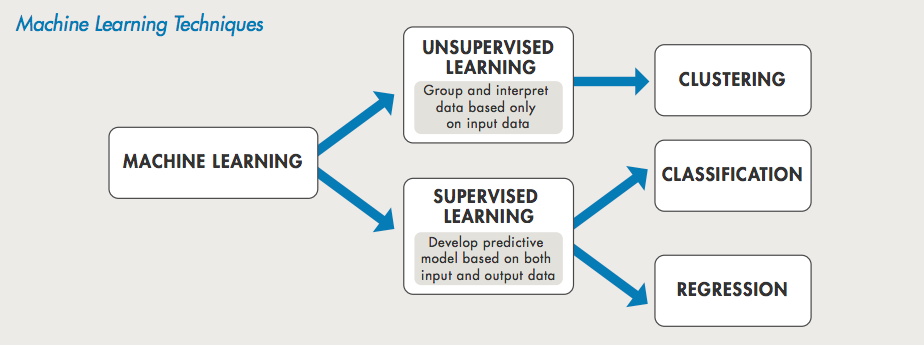
\includegraphics[width=15cm, height=6cm]{images/machinelearning.png}
\caption{Vue globale de Machine learning \cite{key24}}
\label{machinelearning}
\end{figure}

Les algorithmes d'apprentissage peuvent se catégoriser selon le mode d'apprentissage qu'ils emploient :

\subsection{Apprentissage supervisé}
L'apprentissage supervisé (supervised learning en anglais) est une technique d'apprentissage automatique où l'on cherche à produire automatiquement des règles à partir d'une base de données d'apprentissage contenant des « exemples » (en général des cas déjà traités et validés).\\
Une base de données d'apprentissage (ou ensemble d'apprentissage) est un ensemble de couples entrée-sortie $(x_n, y_n)_{1 \leq n \leq N}$ avec $x_n \in X$ et $y_n \in Y $  , que l'on considère être tirées selon une loi sur $ X \times Y $ fixe et inconnue, par exemple $x_n$ suit une loi uniforme et $ y_n = f(x_n) + w_n$ où $w_n$ est un bruit centré. \\\\
On distingue trois types de problèmes solubles avec une méthode d'apprentissage automatique supervisée \cite{key14}:  

\begin{itemize} 
\item $Y \subset \mathbb{R}$  : lorsque la sortie que l'on cherche à estimer est une valeur dans un ensemble continu de réels, on parle d'un problème de régression. La fonction de prédiction est alors appelée un régresseur.
\item $Y = \{ 1, \cdots, I \} $ lorsque l'ensemble des valeurs de sortie est fini, on parle d'un problème de classification, qui revient à attribuer une étiquette à chaque entrée. La fonction de prédiction est alors appelée un classificateur (ou classificateur).
\item Lorsque  $Y$ est un ensemble de données structurées, on parle d'un problème de prédiction structurée, qui revient à attribuer une sortie complexe à chaque entrée. Par exemple, en bio-informatique le problème de prédiction de réseaux d’interactions entre gènes peut être considéré comme un problème de prédiction structurée dans laquelle l'ensemble possible des sorties structurées est l'ensemble de tous les graphes modélisant les interactions possibles \cite{key14}.
\end{itemize}




%si les classes sont prédéterminées et les exemples connus, le système apprend à classer selon un modèle de classement ; on parle alors d'apprentissage supervisé (ou d'analyse discriminante). Un expert (ou oracle) doit préalablement étiqueter des exemples. Le processus se passe en deux phases. Lors de la première phase (hors ligne, dite d'apprentissage), il s'agit de déterminer un modèle des données étiquetées. La seconde phase (en ligne, dite de test) consiste à prédire l'étiquette d'une nouvelle donnée, connaissant le modèle préalablement appris. Parfois il est préférable d'associer une donnée non pas à une classe unique, mais une probabilité d'appartenance à chacune des classes prédéterminées (on parle alors d'apprentissage supervisé probabiliste).\\
%ex. : L'analyse discriminante linéaire ou les SVM en sont des exemples typiques. Autre exemple : en fonction de points communs détectés avec les symptômes d'autres patients connus (les exemples), le système peut catégoriser de nouveaux patients au vu de leurs analyses médicales en risque estimé (probabilité) de développer telle ou telle maladie.

\subsection{Apprentissage non supervisé}
 
Quand le système ou l'opérateur ne disposent que d'exemples, mais non d'étiquettes, et que le nombre de classes et leur nature n'ont pas été prédéterminés, on parle d'apprentissage non supervisé ou clustering. Aucun expert n'est requis. L'algorithme doit découvrir par lui-même la structure plus ou moins cachée des données. Le partitionnement de données, data clustering en anglais, est un algorithme d'apprentissage non supervisé.\\
Le système doit ici — dans l'espace de description (la somme des données) — cibler les données selon leurs attributs disponibles, pour les classer en groupe homogènes d'exemples. La similarité est généralement calculée selon une fonction de distance entre paires d'exemples. C'est ensuite à l'opérateur d'associer ou déduire du sens pour chaque groupe et pour les motifs (patterns en anglais) d'apparition de groupes, ou de groupes de groupes, dans leur « espace ». Divers outils mathématiques et logiciels peuvent l'aider. On parle aussi d'analyse des données en régression (ajustement d'un modèle par une procédure de type moindres carrés ou autre optimisation d'une fonction de coût). Si l'approche est probabiliste (c'est-à-dire que chaque exemple, au lieu d'être classé dans une seule classe, est caractérisé par un jeu de probabilités d'appartenance à chacune des classes), on parle alors de « soft clustering » (par opposition au « hard clustering »).\\
Cette méthode est souvent source de sérendipité(le fait de réaliser une découverte scientifique ou une invention technique de façon inattendue à la suite d'un concours de circonstances fortuit )\\
ex. : Pour un épidémiologiste qui voudrait dans un ensemble assez large de victimes de cancer du foie tenter de faire émerger des hypothèses explicatives, l'ordinateur pourrait différencier différents groupes, que l'épidémiologiste chercherait ensuite à associer à divers facteurs explicatifs, origines géographique, génétique, habitudes ou pratiques de consommation, expositions à divers agents potentiellement ou effectivement toxiques (métaux lourds, toxines telle que l'aflatoxine, etc.) \cite{key13}.

\subsection{Apprentissage semi-supervisé}
Effectué de manière probabiliste ou non, il vise à faire apparaître la distribution sous-jacente des exemples dans leur espace de description. Il est mis en œuvre quand des données (ou « étiquettes ») manquent… Le modèle doit utiliser des exemples non étiquetés pouvant néanmoins renseigner.
Ex. : En médecine, il peut constituer une aide au diagnostic ou au choix des moyens les moins onéreux de tests de diagnostic.
Apprentissage partiellement supervisé 
probabiliste ou non, quand l'étiquetage des données est partiel3. C'est le cas quand un modèle énonce qu'une donnée n'appartient pas à une classe A, mais peut-être à une classe B ou C (A, B et C étant 3 maladies par exemple évoquées dans le cadre d'un diagnostic différentiel) \cite{key13}.
\subsection{Apprentissage par renforcement}l'algorithme apprend un comportement étant donné une observation. L'action de l'algorithme sur l'environnement produit une valeur de retour qui guide l'algorithme d'apprentissage \cite{key13}.
ex. : L'algorithme de Q-learning est un exemple classique.
\subsection{Apprentissage par transfert}
L’apprentissage par transfert peut être vu comme la capacité d’un système à reconnaître et appliquer des connaissances et des compétences, apprises à partir de tâches antérieures, sur de nouvelles tâches ou domaines partageant des similitudes. La question qui se pose est : comment identifier les similitudes entre la ou les tâche(s) cible(s) et la ou les tâche(s) source(s), puis comment transférer la connaissance de la ou des tâche(s) source(s) vers la ou les tâche(s) cible(s) ? \cite{key13}
\subsection{Notion de dataset}
Le dataset est l'ensemble des données utilisé pour entraîner un modèle. Il existe deux types de jeux de données (dataset) généraux. Jeux étiqueté et jeux sans étiquette \cite{key15}.
\subsection{Training Set and Test Set}
Dans l'apprentissage automatique, un jeu de données universel inconnu est supposé exister, qui contient toutes les paires de données possibles ainsi que leur distribution de probabilité d'apparition dans le monde réel. Alors que dans les applications réelles, ce que nous avons observé est seulement un sous-ensemble de l'ensemble de données universel en raison du manque de mémoire ou d'un autre inévitable les raisons. Cet ensemble de données acquises s'appelle l'ensemble d'apprentissage \textbf{(Training Set)} et est utilisé pour apprendre les propriétés et la connaissance de l'ensemble de données universel. Afin d'examiner la performance de l'apprentissage, un autre ensemble de données peut être réservé pour le test, appelé ensemble de test ou données de test \textbf{(Test Set)} \cite{key15}.\\
%\begin{itemize}
%\item Dataset étiqueté: $\mathbb{D}: X = \{x^{(n)} \in \mathbb{R}^ $ 
%\end{itemize}


Le machine learning est un champ d'études vaste, c'est un domaine de recherche. Dans ce rapport nous ne pouvons pas aborder tous les concepts découlant du machine learning mais nous allons considérer un sous-ensemble de concepts que nous avons utilisés pour le développement de notre projet. Dans notre cas, c'est un problème de classification qui fait partie de l'apprentissage supervisé. C'est comme l'exemple des courriers spam et anti-spam que nous avons pris dans l'introduction de cette section. Le problème est de décider est-ce que le patient doit retourner chez lui ou s'il doit rester à l'hôpital après une arthoplastie. Si la réponse est vraie le patient reste à l'hôpital sinon il retourne chez lui. Il faut toujours garder en esprit que cette décision est importante pour un centre orthopédique car elle peut réduire ou augmenter le coût budgétaire.   

\section{Problème de Classification}

Dans l'apprentissage automatique et les statistiques, le problème de classification est le problème d'identifier lequel d'un ensemble de catégories (sous-population) appartient à une nouvelle observation, sur la base d'un ensemble de données contenant des observations (ou instances) dont la composition est connue \cite{key16}.\\

Voici quelques exemples de problèmes de classification. Nous avons déjà parlé de la classification du spam par courrier électronique comme exemple de problème de classification. Un autre exemple serait le classement des transactions en ligne. Donc, si vous avez un site Web qui vend des trucs et si vous voulez savoir si une transaction particulière est frauduleuse ou non, si quelqu'un utilise une carte de crédit volée ou a volé le mot de passe de l'utilisateur. Si la transaction est frauduleuse, on retourne 1 comme valeur sinon l'algorithme retourne 0.\\
0 est aussi appelé la classe négative, et 1 la classe positive, et ils sont parfois aussi désignés par les symboles "-" et "+".\\

Dans notre projet, le problème est un problème de classification binaire parce qu'on doit décider si oui ou non le patient reste à l'hôpital après une intervention chirurgicale. Si le patient reste, la valeur de la classe est positive (c'est-à-dire 1), s'il ne reste pas ou il est renvoyé, la valeur de la classe est négative (c'est-à-dire 0).

\subsection{Mesure de performance des algorithmes de classification}
L'évaluation de la performance des méthodes d'apprentissage automatique est aussi cruciale que l'algorithme lui-même, car il identifie les forces et les faiblesses de chaque algorithme d'apprentissage. Différentes mesures de performance sont utilisées pour évaluer différents algorithmes d'apprentissage automatique. Pour l'instant, nous allons nous concentrer sur ceux utilisés pour les problèmes de classification. Quelques metrics que nous pouvons utiliser pour évaluer la performance des problèmes de classification sont Log-Loss, Accuracy, AUC(Area under Curve) etc. Ils font partie des plus communs mais nous pouvons créer des metrics personnalisés en fonction de nos besoins \cite{key17}.\\

Les metrics que vous choisissez pour évaluer votre modèle d'apprentissage automatique sont très importantes. Le choix des paramètres influence la façon dont la performance des algorithmes d'apprentissage automatique est mesurée et comparée. Pour ne pas perdre plus de temps, voyons ce que sont quelques metrics que nous avons utilisé dans notre projet.

\subsection{Matrice de confusion}
La matrice de confusion \textbf{(Confusion Matrix en anglais)} est l'une des mesures les plus intuitives et les plus faciles (à moins bien sûr, vous n'êtes pas confus) utilisées pour trouver l'exactitude et la précision du modèle. Il est utilisé pour les problèmes de classification où la sortie peut être de deux types ou plus de classes \cite{key17}.\\

La figure \ref{confusionmatrix} est une représentation de la matrice de confusion. La valeur actuelle (Actual value) représente la vraie valeur de l'étiquette tandis que la valeur prédite (Predicted value) représente la valeur retournée par le modèle machine learning. 
\paragraph*{True Positives (TP):}
Les vrais positifs sont les cas où la classe réelle du point de données était 1 (Vrai) et la prédiction est également 1 (Vrai)
\paragraph*{True Negatives (TN):}
Les vrais négatifs sont les cas où la classe réelle du point de données était 0 (Faux) et la prédiction est également 0 (Faux)

\begin{figure}[h]
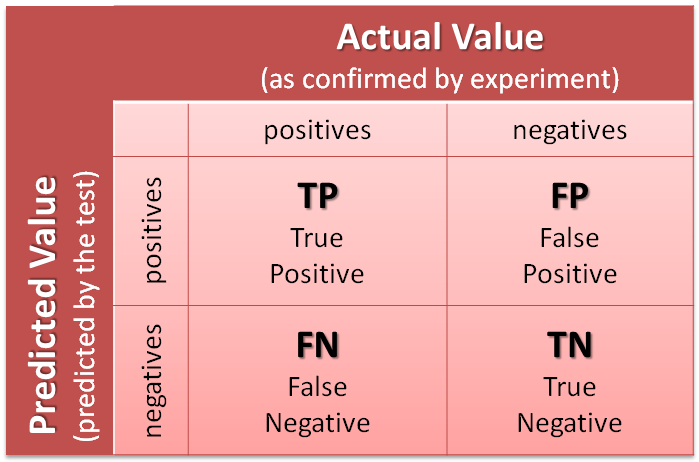
\includegraphics[width=14cm, height=7cm]{images/confusionmatrix.png}
\caption{Confusion Matrix representation \cite{key25}}
\label{confusionmatrix}
\end{figure}

\paragraph*{False Positives (FP):}
Les faux positifs sont les cas où la classe réelle du point de données était 0 (Faux) et la prédiction est 1 (Vrai). Faux parce que le modèle a prédit incorrectement et positivement parce que la classe prédite était positive. (1)
\paragraph*{False Negatives (FN):}
Les faux négatifs sont les cas où la classe réelle du point de données était 1 (Vrai) et la prédiction est 0 (Faux). Faux parce que le modèle a prédit incorrectement et négativement parce que la classe prédite était négative. (0)



\subsection{Calcul de certains metrics de classification à partir de la matrice confusion}

La matrice de confusion en soi n'est pas une mesure de performance en tant que telle, mais presque toutes les métriques de performance sont basées sur la matrice de confusion et les nombres qui s'y trouvent. Nous allons voir comment utiliser la matrice de confusion pour calculer quelques metrics de classification \cite{key17}.

\begin{enumerate}
\item \textbf{Accuracy:}
L'exactitude \textbf{(Accuracy en anglais)} dans les problèmes de classification est le nombre de prédictions correctes faites par le modèle sur toutes les prédictions faites.
$\textnormal{Accuracy} = \frac{TP+TN}{TP+ FP + FN + TN} $

\item  \textbf{Precision:} 
La précision permet de répondre à la question suivante : Quelle proportion d'identifications positives était effectivement correcte ?
$\textnormal{Precision} = \frac{TP}{TP+ FP} $

\item \textbf{Recall or Sensitivity:}
Le rappel permet de répondre à la question suivante : Quelle proportion de résultats positifs réels a été identifiée correctement ?
$\textnormal{Recall} = \frac{TP}{TP+ FN} $
 
 \item \textbf{F1-score:}
 Nous ne voulons pas vraiment avoir à la fois la précision et le rappel dans nos poches chaque fois que nous faisons un modèle pour résoudre un problème de classification. Donc, il est préférable que nous puissions obtenir un seul score qui représente à la fois la précision (P) et le rappel (R)
 
 $ \textnormal{F1score} = \frac{ 2 }{\frac {1}{\textnormal{precision}} +  \frac {1}{\textnormal{recall}}  } = 2 \times \frac{\textnormal{precision} \times \textnormal{recall}} { \textnormal{precision} + \textnormal{recall} } = \frac{TP} {TP + \frac{FN+FP} {2} } $
 
 \item \textbf{ROC-AUC:}
Une courbe ROC (receiver operating characteristic) est un graphique représentant les performances d'un modèle de classification pour tous les seuils de classification. Cette courbe trace le taux de vrais positifs \textbf{(True Positifs en anglais)} en fonction du taux de faux positifs \textbf{(False Positifs en anglais)} \cite{key18}.
\end{enumerate}

\section{Classes déséquilibrées}

Nous terminerons le chapitre sur la classification en abordant un sujet très important en machine learning, surtout dans le problème de la classification qui est "\textit{Jeux de données déséquilibré}" \textbf{(Imbalanced datasets or Imbalanced Classification or Imbalanced Classes, ses appellations en anglais)}. C'est un problème très commun en machine learning, spécialement en classification. Nous abordons ce sujet parce que c'était l'une des principales difficultés de notre projet. \\

Une distribution de classe déséquilibrée est un scénario où le nombre d'observations appartenant à une classe est significativement inférieur à celui des autres classes. 
Ce problème prédomine dans les cas où la détection d'anomalies est cruciale comme le vol d'électricité, les transactions frauduleuses dans les banques, l'identification de maladies rares, etc. Dans ce cas, le modèle prédictif développé avec des algorithmes conventionnels pourrait être biaisé et inexact.\\
Cela arrive parce que les algorithmes d'apprentissage automatique sont généralement conçus pour améliorer la précision en réduisant l'erreur. Ainsi, ils ne tiennent pas compte de la répartition / proportion des classes ou de l'équilibre des classes \cite{key19}.\\

Plusieurs techniques ont été proposées pour manipuler les classes déséquilibrées. Voyons un bref résumé de quelques-unes d'entre elles  \cite{key19}:
\subsection{Random Under-Sampling:}
Le Random Under-Sampling vise à équilibrer la distribution des classes en éliminant de manière aléatoire les exemples de classes majoritaires. Ceci est fait jusqu'à ce que les instances de la majorité et de la classe minoritaire soient équilibrées.
\subsection{Random Over-Sampling:}
Le Random Over-Sampling augmente le nombre d'instances dans la classe minoritaire en les reproduisant aléatoirement afin de présenter une représentation plus élevée de la classe minoritaire dans l'échantillon.
\subsection{Cluster-Based Over Sampling:}
Dans ce cas, l'algorithme de clustering K-means est appliqué indépendamment aux instances de classe minoritaire et majoritaire. Cela permet d'identifier les clusters dans l'ensemble de données. Par la suite, chaque grappe est suréchantillonnée de sorte que tous les clusters de la même classe ont un nombre égal d'instances et toutes les classes ont la même taille.
\subsection{Synthetic Minority Over-sampling Technique(SMOTE):}
Cette technique est suivie pour éviter le surapprentissage qui se produit lorsque des répliques exactes d'instances minoritaires sont ajoutées à l'ensemble de données principal. Un sous-ensemble de données est pris à partir de la classe minoritaire à titre d'exemple, puis de nouvelles instances similaires synthétiques sont créées. Ces instances synthétiques sont ensuite ajoutées à l'ensemble de données d'origine. Le nouvel ensemble de données est utilisé comme un échantillon pour former les modèles de classification.
\subsection{Modified synthetic minority oversampling technique (MSMOTE):}
C'est une version modifiée de SMOTE. SMOTE ne tient pas compte de la distribution sous-jacente de la classe minoritaire et des bruits latents dans l'ensemble de données. Pour améliorer les performances de SMOTE, une méthode modifiée MSMOTE est utilisée.\\

Dans notre projet nous avons opté pour la technique de SMOTE parce qu'elle permet d'atténuer le problème de sur-adaptation \textbf{(overfitting en anglais)} causé par le sur-échantillonnage aléatoire \textbf{(random oversampling, en anglais)} \\

\section{Conclusion}
Le chapitre 2 a présenté une vue générale sur les différents concepts utilisés en sciences de données et en machine learning. On a donné une brève définition de chaque concept tout en essayant d'être le plus clair et précis possible. Nous avons vu un sous-ensemble de ces concepts car ces champs d'études sont très vastes et contiennent beaucoup de choses intéressantes, mais nous avons mis accent sur ce qui nous intéresse pour notre projet. Par exemple notre projet est un problème de classification en machine learning, pour cela nous avons dédié une section à l'étude brève de classification. Aussi notre dataset est déséquilibré, par conséquent nous avons eu une section qui montre comment manipuler les classes déséquilibrées et les différentes techniques de manipulation. Le chapitre 3 qui suit présentera les détails techniques de notre projet, le but est de faire sortir les différentes étapes que nous avons suivies pour arriver à un produit fini et utilisable.

 




%\begin{table}[htp]
%\caption{Confusion Matrix}
%\begin{center}
%\begin{tabular}{|c|c|}
%
%\hline
%
%\hline
%
%\hline
%
%\hline
%
%\end{tabular}
%\end{center}
%\label{default}
%\end{table}%

    %%%%%%%%%%%%%%%%%%%. Chapitre 3 %%%%%%%%%%%%%%%%%%%%%%%%%%%%%%%%%%%%%%%%%%%%%%%%%%%%%%


\newpage

\chapter{Approche: Construction du modèle machine learning}
\section{Introduction}

Le développement du modèle est la première grande phase de l'implémentation de notre solution. Le modèle estimateur (meilleur modèle entrainé en fonction de notre ensemble de données) va être utilisé pour introduire la deuxième phase, celle de la création de l'API Ortho. Comme nous avons déjà vu dans l'introduction le diagramme de cas d'utilisation du système machine learning. Nous proposons maintenant un diagramme de classe (figure \ref{MLClassDiag}) qui répond aux différentes exigences que nous avons décrites. Nous tenons à souligner que dans notre diagramme de classe nous ne prenons pas en compte les classes prédéfinies dans les librairies de Python. Par exemple le \textbf{DataFrame} est une classe prédéfinie dans la librairie \textbf{pandas}. Nous l'utilisons dans notre classe \textbf{Gather} mais elle n'est pas définie dans notre diagramme de classe.  \\ 

%Pour développer notre projet, nous avons fait le cycle complet d'un data scientist. Depuis l'obtention des données jusqu'au déploiement d'un système en production. Dans ce chapitre nous allons parcourir toutes les étapes du développement de notre projet. Chaque section représente une étape du projet. Il peut y avoir de petites définitions pour éclairer certains thèmes que nous n'avons pa pu aborder dans le chapitre sur le \textbf{Contexte Théorique}.


Dans les sections qui suivent nous allons voir les différentes étapes d'implémentation de notre système machine learning. Nous commençons d'abord par l'obtention des données, pour ensuite les explorer, ensuite les nettoyer, les transformer et enfin les modéliser. 

\begin{figure}[p]
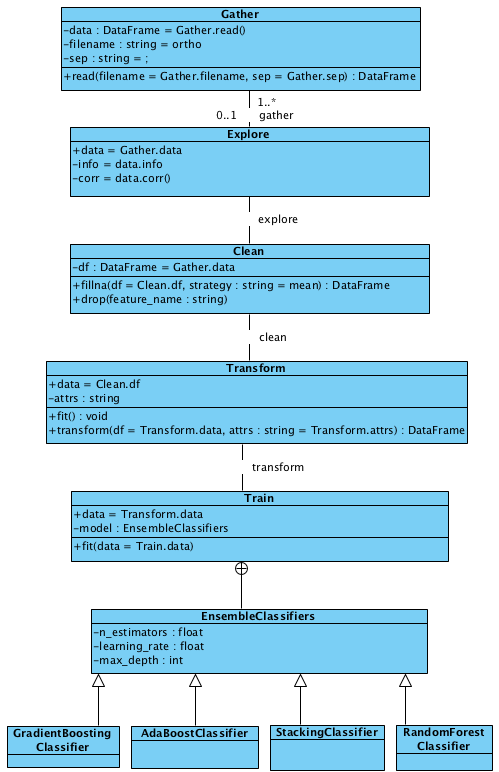
\includegraphics[width=13cm, height=19cm]{images/MLClassDiag.png}
\caption{Class diagram of our machine learning system}
\label{MLClassDiag}
\end{figure}
\newpage


\section{Obtention des données}
Nos données proviennent du département orthopédique de l'université de Seattle, Washington, États-Unis. Elles sont au nombre de 2718 files et 92 colonnes. Nous les utilisons comme données historiques (\textit{historical data, en anglais}) dans le cadre du développement de notre modèle de machine learning. 
Une fois qu'on décide à attaquer un problème de machine learning, la première chose à faire est d'explorer toutes les pistes possibles pour récupérer les données. En effet, les données constituent l'expérience, les exemples qu'on va fournir à notre algorithme de machine learning afin qu'il puisse apprendre et devenir plus performant.\\ 

Les données que nous utilisons dans ce projet proviennent de la compagnie pour laquelle nous faisons le stage. Cette dernière les avait obtenues de l'université Seattle, Washington, USA. Les données sont disponibles dans un fichier d'extension csv et hébergées sur le serveur de la compagnie. Par conséquent, nous avons un accès direct aux données sans avoir besoin de les télécharger à partir d'un dépôt de Machine Learning. \\

Comme vous pouvez remarquer dans la classe diagramme du machine learning (figure \ref{MLClassDiag}), on a implémenté un classe nommant \textbf{Gather}. Celle-ci nous permet d'obtenir les données brutes à travers la méthode \textbf{read} qui prend en paramètre un nom de fichier (\textbf{filename}) et un séparateur (\textbf{sep}). Le fichier contient toutes les données disponibles pour la construction du modèle et le séparateur permet de préciser comment les colonnes sont séparées entre elles, dans notre cas c'est un point virgule (\textbf{;}) qui les sépare.

Après avoir obtenu les données, il faut maintenant les explorer pour avoir des idées claires sur l'ensemble des données. La section suivante est l'étape d'exploration des données, les données obtenues à la classe Exploration de données. 

\section{Exploration des données}

Le but de l'analyse exploratoire est de «connaître» l'ensemble de données. Si vous le faites à l'avance, le reste du projet sera beaucoup plus fluide, de trois façons principales \cite{key20}:
\begin{enumerate}
\item Vous obtiendrez des conseils précieux pour le nettoyage des données \textbf{(Data Cleaning en anglais)} qui peuvent faire ou défaire vos modèles.
\item Vous penserez à des idées pour l'ingénierie des fonctionnalités \textbf{(Feature Engineering en anglais)} qui peuvent prendre vos modèles de bonne à grande.
\item Vous obtiendrez une «idée» de l'ensemble de données, ce qui vous aidera à communiquer les résultats et à avoir un impact plus important.
\end{enumerate}

Pour l'analyse exploratoire de nos données, Tout d'abord, nous commençons par une analyse basique de l'ensemble de nos données \textbf{(dataset in english)}. La table \ref{tab:dataset} donne une description de notre dataset utilisé pour notre projet et la figure \ref{fig:samplesdataset} donne une vue de notre ensemble de données, leur représentation, et leurs valeurs possibles. Si nous nous référons à notre classe diagramme \ref{MLClassDiag}), c'est l'attribut info de la classe Explore qui nous fournit les informations sur notre dataset. La méthode head nous retourne les cinq premières lignes du jeu de données.

Voyons une brève description de chaque composante du dataset après une analyse basique de notre exploration:

\paragraph*{Number of Features :} Représente le nombre totale de features ou colonnes de notre dataset. Les features sont importants pour un modèle de machine learning puisque le modèle les utilise pour prédire des événements. Dans l'annexe A, La table \ref{tab:dt} donne une description de tous les features de notre dataset. Le nombre total des features est 92.  La colonne \textbf{Feature name} représente le nom de chaque colonne. La colonne \textbf{datatype} représente le type de données et les colonnes. Et les colonnes \textbf{non-null} et \textbf{null} représentent respectivement le nombre d'échantillons non-nulls et le nombre d'échantillons nulls. Référez-vous à la table \ref{tab:dt}, pour prendre connaissance des nom de colonnes car nous allons les utiliser plus tard. 



\begin{table}[h]
\centering
\begin{tabular}{|l|c|c|c|c|c|}
\hline
Number of Features & 92 \\
\hline
Number of Observations & 2718\\
\hline
Number of Numerical Features & 87\\
\hline
Number of Categorical Features & 5\\
\hline
Target value & Discharge\\
\hline

\end{tabular}
\caption{Gives a description of our dataset}
\label{tab:dataset}
\end{table}

\begin{figure}[h]
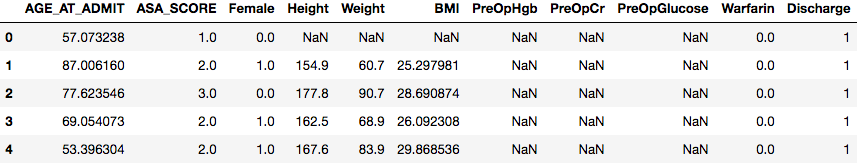
\includegraphics[width=18cm]{images/examplesfeatures.png}
\caption{An overview of raw data from our dataset}
\label{fig:samplesdataset}
\end{figure}


\paragraph*{Number of Observations :} Représente le nombre d'échantillons \textbf{(samples or rows en anglais)} de notre ensemble de données. 

\paragraph*{ Numerical Features :} Ce sont les caractéristiques numériques de notre dataset. Les valeurs continues de notre dataset.

\paragraph*{ Categorical Features :} Ce sont les features qui viennent sous forme de texte. Plus loin dans la section de la transformation, nous convertirons ces features en données numériques car la plupart des algorithmes de machine learning ne reconnaissent pas les données discrètes ou textuelles.

\paragraph*{ Target value :} C'est l'étiquette (\textbf{label or target en anglais)} de notre ensemble de données. L'étiquette est une valeur très importante pour les algorithmes de classification car elle permet d'évaluer la valeur booléenne d'une décision. Dans notre cas c'est le \textit{Discharge} qui permet de dire si oui ou non le patient doit rester à l'hôpital pour une réadaptation. \\

\begin{table}[h]
\centering
\begin{tabular}{| l | c |}
\hline
\textbf{Target's name} & Discharge \\
\hline
\textbf{Total positive classes} & 2421 \\
\hline
\textbf{Percentage positive classes} & 89.072848 \% \\
\hline
\textbf{Negative classes} & 297 \\
\hline
\textbf{Percentage negative classes} & 10.927152 \% \\
\hline
\textbf{Total classes} & 2718 \\

\hline
\end{tabular}
\caption{Important details about target value}
\label{tab:target}
\end{table}

La table \ref{tab:target}, quant à elle, c'est la représentation de notre variable target value. Dans le dataset, elle s'appelle \textit{Discharge}. On peut remarquer que les classes positives sont significativement plus nombreuses que les classes négatives, ce qui produit un déséquilibre au niveau du dataset. Nous avons déjà discuté dans la section\textit{ "Classes déséquilibrées"}, les différentes techniques pour équilibrer les classes déséquilibrées.

\subsection{Correlation entre les données}
Nous terminons la section d'exploration de données avec les corrélations. Les corrélations nous permettent d'examiner les relations entre les entités numériques et d'autres entités numériques \textbf{(Numerical features en anglais)}. La corrélation est une valeur comprise entre -1 et 1 qui représente à quel point deux entités se déplacent à l'unisson \cite{key20}. \\

Une corrélation positive signifie que lorsqu'une caractéristique augmente, l'autre augmente. Par exemple. Le BMI d'un patient et son poids\textbf{ (Weight dans le dataset)}.\\

La corrélation négative signifie que lorsqu'une caractéristique augmente, l'autre diminue. Par exemple. heures consacrées à l'étude et nombre de participants. Les corrélations proches de -1 ou 1 indiquent une relation forte. Les plus proches de 0 indiquent une relation faible. 0 indique aucune relation.

\begin{figure}[h]
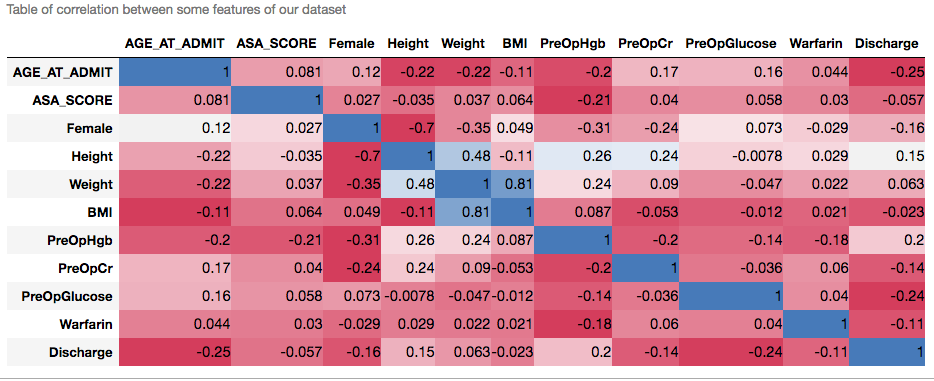
\includegraphics[width=17.5cm, height =7cm]{images/correlation.png}
\caption{General view of the correlation between some features of our dataset}
\label{fig:correlation}
\end{figure}

La figure \ref{fig:correlation} nous donne une idée comment nos variables sont corrélées entre elles. Par exemple, le poids \textbf{ (Weight dans le dataset)} et le \textbf{BMI} ont une correlation de 0.81 très proche de 1. On peut déduire que les patients qui ont leur BMI plus élevé sont les plus pesants. L'objectif de la correlation est de gagner en intuition sur les données, ce qui nous aidera tout au long du flux de travail.\\ 

Pour calculer la correlation, nous avons utilisé la méthode \textbf{corr} de  la classe \textbf{Explore}. Nous avons passé un peu de style comme paramètre pour avoir les couleurs.  \\
 
Après avoir exploré les données et acquérir suffisamment de connaissance sur notre ensemble de données, c'est le temps maintenant de les nettoyer. La section qui suit montre comment nous avons procédé pour nettoyer notre dataset.

\section{Nettoyage des données}
Le nettoyage des données \textbf{(Data cleaning en anglais)} est l'une de ces choses que tout le monde fait mais dont personne ne parle vraiment. Bien sûr, ce n'est pas la partie la plus intéressante de l'apprentissage automatique. Et non, il n'y a pas de trucs cachés et de secrets à découvrir.

Cependant, un nettoyage correct des données peut faire ou défaire notre projet. Les spécialistes des données professionnelles consacrent généralement une très grande partie de leur temps à cette étape. En fait, si vous avez un jeu de données correctement nettoyé, même des algorithmes simples peuvent apprendre des informations impressionnantes à partir des données! \cite{key21}.

\subsection{Observations indésirables} La première étape du nettoyage des données consiste à supprimer les observations indésirables de votre jeu de données. Cela inclut des observations en double \textbf{(Duplicate observations)} ou non pertinentes \textbf{(Irrelevant observations)} \cite{key21}.

\subsection{Duplicate observations :} Les observations en double surviennent le plus souvent lors de la collecte de données, notamment lorsque vous combinez des ensembles de données provenant de plusieurs endroits, capturez les données et recevez des données de clients / autres départements \cite{key21}.

\subsection{Irrelevant observations :} Les observations non pertinentes sont celles qui ne correspondent pas vraiment au problème spécifique que vous essayez de résoudre \cite{key21}. \\

Dans notre projet, nous avons trouvé beaucoup de données impertinentes. Par exemple. pendant la phase d'exploration nous avons trouvé que le "\textbf{Weight}" est une donnée impertinente car elle très corrélée avec le "\textbf{BMI}". On a décidé de maintenir le \textbf{BMI} et de laisser tomber le \textbf{"Weight"}.  De la même manière nous nous rendons compte que le \textbf{"RawDX"} et \textbf{"GHOA}" étaient les mêmes données sauvegardées sous des formes différentes. Et on a maintenu le \textbf{"RawDX"} et laissé tomber le \textbf{"GHOA"}. La méthode \textbf{drop} de la classe \textbf{Clean} est utilisée pour supprimer les features non pertinents.  

\subsection{Données manquantes}
Les données manquantes \textbf{(Missing data en anglais)} sont un problème trompeur dans l'apprentissage automatique appliqué. Tout d'abord, juste pour être clair, vous ne pouvez pas simplement ignorer les valeurs manquantes dans un ensemble de données. Vous devez les gérer d'une manière ou d'une autre pour la raison très pratique que la plupart des algorithmes n'acceptent pas les valeurs manquantes.\\

Les deux stratégies les plus couramment recommandées pour traiter les données manquantes sont les suivantes \cite{key21}:
\begin{enumerate}
\item Suppression des observations qui ont des valeurs manquantes \textbf{(Dropping en anglais)}
\item Imputation des valeurs manquantes en fonction d'autres observations \textbf{(Imputing en anglais)}
\end{enumerate}

Après avoir essayé les deux recommandations, nous avons constaté que le \textbf{"imputing"} nous donne de meilleurs résultats. Pour arriver à cette affirmation, nous avons essayé plusieurs modèles avec leurs différentes évaluations. Il faut souligner que notre dataset a de beaucoup de valeurs nulles. C'est la deuxième difficulté du projet après le déséquilibre au niveau du dataset. \\

Il est important de préciser que dans le  \textbf{"imputing"}, il y a plusieurs méthodes de remplissage. On peut remplir avec la valeur "\textbf{zéro (0})", la valeur moyenne "\textbf{mean}" ou la valeur moyenne "\textbf{median}". Encore, nous avons opté de remplir avec la valeur moyenne "\textbf{mean}", car elle nous a donné de meilleurs résultats. La méthode \textbf{fiilna} de la classe \textbf{Clean} est utilisée pour remplir les données manquantes. Elle prend un jeu de données et la stratégie de remplissage en paramètres et elle retourne un jeu données sans données manquantes. \\

La prochaine section va être l'étape de transformation ou le feature engineering. Une fois que nos données sont nettoyées et il n'y a pas de données vides, on peut les transformer pour en avoir de nouvelles beaucoup plus pertinentes. 

\section{Feature Engineering}

L'ingénierie des caractéristiques \textbf{(Feature Engineering en anglais)} consiste à créer de nouvelles entités en entrée à partir de celles qui existent déjà. En général, vous pouvez considérer le nettoyage des données comme un processus de soustraction et l'ingénierie des fonctionnalités comme un processus d'ajout. C'est souvent l'une des tâches les plus précieuses qu'un data scientist puisse faire pour améliorer les performances du modèle, et ce, pour trois grandes raisons \cite{key22}:

\begin{enumerate}
\item Vous pouvez isoler et mettre en évidence les informations clés, ce qui aide vos algorithmes à se concentrer sur ce qui est important.
\item Vous pouvez apporter votre propre expertise de domaine.
\item Plus important encore, une fois que vous comprenez le «vocabulaire» de l'ingénierie des caractéristiques, vous pouvez apporter l'expertise de domaine d'autres personnes!
\end{enumerate}

Le feature engineering est l'étape qui précède la modélisation. Il prend en entrée le jeux de données brutes et produit en sortie un jeux de données préparé pour l'étape de la modélisation. Le modèle prend en entrée le jeux de données produit par le processus du feature engineering. \\ 

Nous avons fait notre feature engineering en deux étapes: 
\begin{enumerate}
\item Premièrement, les features \textbf{Dx1, Dx2, Dx3 } qui existent déjà dans notre dataset doivent être combinés entre eux pour créer un nouveau feature appelé \textbf{degree\_dx} qui est le niveau général diagnostique du patient. Nous soulignons que  \textbf{Dx1, Dx2, Dx3} représentent respectivement: premier niveau diagnostique, deuxième niveau diagnostique et troisième niveau diagnostique du patient. En combinant ces trois diagnostiques, nous créons un niveau général  diagnostique du patient. \\
\textbf{Logique de création : } On regroupe ces colonnes (\textbf{Dx1, Dx2, Dx3 }) suivants la logique si les 3 sont presents (c'est-à-dire si les 3 ont valeurs non-null), on donne la valeur de 3; si uniquement DX2 et DX1 sont présents, on donne la valeur de 2; si uniquement DX1 on donne la valeur de 1 si aucune valeur n'est présente, on donne la valeur 0. Le feature résultant se nomme  \textbf{degree\_dx}
\item Deuxièment, nous créons un nouvel autre feature appelé \textbf{medcond} qui détermine les conditions médicales du patient. Nous nous basons sur l'ensemble de caractéristiques pré-opératoires du patient. Par exemple son niveau de glucose, les quantités d'hémoglobine blanches et d'hémoglobines rouges. Ces features sont au nombre de 46 au total.\\
\textbf{Logique de création : } On prend toutes les colonnes de conditions médicales (\textbf{PreOpHgb}  à \textbf{Depression}, ils sont au nombre de 46 dans le dataset) : On donne la valeur 1 lorsqu'on trouve une valeur non-nulle à chacune des conditions sauf pour les colonnes suivantes :
\begin{itemize}
\item On donne la valeur 2 pour les colonnes suivantes: [\textbf{PreOpHgb, PreOpGlucose, pulm circ, other neuro, chronic pulm}]
\item On donne la valeur 3 pour les colonnes suivantes [\textbf{PreOpC, Paralysis, renal failure, liver failure}]
\end{itemize}


\end{enumerate}

La classe Transform de notre diagramme de classe fait toutes les transformations que nous venons de décrire dans cette section. La méthode \textbf{transform} prend en paramètre le jeu de données nettoyé et les attributs à transformer et elle retourne un jeu de données transformé lequel nous allons utiliser comme entrée de l'étape suivante sur la modélisation. 


 


\section{Modélisation des données}

La modélisation est un processus d'entrainement de modèles. Il consiste à décrire comment choisir le meilleur modèle qui s'adapte à la problématique qu'on étudie et les raisons pour lesquelles le modèle choisi est meilleur. Ici, meilleur modèle ne veut pas dire qu'un algorithme est meilleur qu'un autre mais tout dépend du cas qu'on étudie.\\

Toutes les étapes que nous venons de détailler dans les sections précédentes constituent des étapes préparatoires pour la modélisation. Dans l'étape d'exploration de données, nous nous sommes rendus compte que notre ensemble de données était déséquilibré. \\ 

Puisque notre ensemble de données est déséquilibré, nous ne pouvons pas utiliser les algorithmes de classification simples tel que LogisticRegression, TreeDecisionClassifier, LinearClassifier etc. Nous avons utilisé l'approche des méthodes d'ensemble qui consiste à combiner plusieurs classificateurs simples pour donner un classificateur fort. L'image \ref{ensemble} donne une approche générale sur le fonctionnement et la construction des méthodes d'ensemble. \textbf{Data} représente l'ensemble de données d'origine, (\textbf{C1, C2, ... , Cn}) sont les différents algorithmes de classification faibles qu'on combine pour donner en entrée à \textbf{Vote Classifier}. \textbf{Strong Classifier} est l'algorithme de classification fort qu'on obtient. \\

Dans le chapitre sur \textit{"Contexte théorique"} nous avons vu comment manipuler les données déséquilibrées en ré-échantillonnant \textbf{(resampling en anglais)} les données d'origine pour fournir des classes équilibrées. Nous avons vu toutes les avantages à utiliser les techniques SMOTE que les autres. Dans la sous-section qui suit sur la modélisation, nous allons brièvement examiner une autre approche, à savoir la modification des algorithmes de classification existants pour les rendre appropriés aux ensembles de données déséquilibrés. 



\subsection{Méthodes d'ensemble}

L'objectif principal de la méthodologie d'ensemble \textbf{(Ensemble methods en anglais)} est d'améliorer la performance des classificateurs uniques. L'approche consiste à construire plusieurs classificateurs à deux étapes à partir des données originales, puis à agréger leurs prédictions \cite{key1}. Les méthodes d'ensemble sont nombreuses, mais nous allons brièvement définis les trois plus importantes: Bagging, Boosting et Random Forest. 

\begin{figure}[h]
	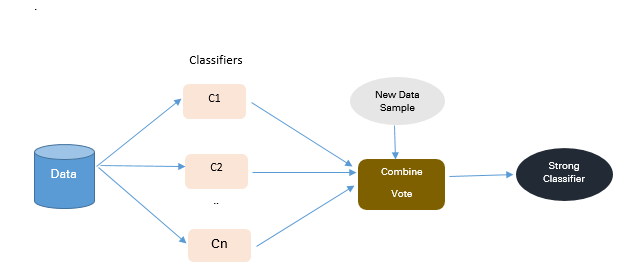
\includegraphics{images/ensemble.png}
	\caption{Approach to Ensemble based Methodologies \cite{key19} }
	\label{ensemble}
\end{figure}

\subsubsection{Bagging}
Bagging (Bootstrap aggregating) est une approche de construction d'ensemble qui 
utilise différents sous-ensembles de données d’apprentissage avec une  méthode  de classification unique.  Étant  donné  un  ensemble  d’apprentissage  de  taille \textbf{t}, Bagging attire des instances aléatoires \textbf{t} de l'ensemble de données avec remplacement (à l'aide d'une distribution uniforme). Ces \textbf{t} instances sont apprises, et ce processus est répété plusieurs fois. Étant donné que le tirage au sort est effectué avec remplacement, les   instances   tirées   contiendront des   doublons   et   des   omissions   par   rapport   à l'ensemble  d'apprentissage initial.  Chaque  cycle  à  travers  le  processus  aboutit  à  un classificateur.  Après  la  construction  de  plusieurs  classificateurs,  les  sorties  de  chaque classificateur sont combinés pour produire la prédiction finale \cite{key27}. 
%Méthodes parallèles (ensachage, forêt aléatoire) dont le principe est de faire la moyenne de plusieurs prédictions dans l'espoir d'un meilleur résultat suite à la réduction de la variance de l'estimateur moyen.
\subsubsection{Boosting}
Une  autre  approche  appelée  «Boosting»  utilise  également une  méthode d'apprentissage  unique  avec  différents  sous-ensembles  de  données  d’apprentissage. Sa structure globale est similaire à celle de la méthode Bagging, à la différence qu’elle  conserve  la  trace  de  la  performance  de  l'algorithme  d'apprentissage  et  se concentre  sur  les  cas  qui  ne  sont  pas  correctement  appris.  Au  lieu  de  choisir  les instances \textbf{t} d’apprentissage à l'aide d'une distribution uniforme de manière aléatoire, les exemples d’apprentissage sont sélectionnés en favorisant les instances quine sont pas  bien  classées.  Après  plusieurs  cycles,  la  prédiction  est  réalisée  selon  un  vote pondéré des prédictions de chaque classificateur. Ainsi, les poids sont proportionnels à la précision de chaque classificateur sur son ensemble d'apprentissage. L’algorithme le plus connu de l’approche Boosting, appelée « AdaBoost » \cite{key27}.
\subsubsection{Stacking}
Le stacking est similaire au boosting: vous appliquez également plusieurs modèles à vos données d'origine. La différence ici est, cependant, que vous n'avez pas juste une formule empirique pour votre fonction de poids, plutôt que vous introduisez un méta-niveau et utilisez un autre modèle / approche pour estimer l'entrée avec les sorties de chaque modèle pour estimer les poids ou , en d'autres termes, pour déterminer quels modèles fonctionnent bien et ce qui est mal donné ces données d'entrée \cite{key28}. 
\subsubsection{Random Forest}
Les forêts aléatoires(plus connus sous \textbf{Random Forest}) sont une combinaison d'arbres  de  décision,  où  chaque  arbre  dépend  des  valeurs  d'un  vecteur  aléatoire indépendamment échantillonné et avec la même distribution pour tous les arbres de la forêt.L'erreur  de  généralisation  d'une  forêt  d'arbres  dépend  de  la  force  des  arbres individuels  dans  la  forêt  et  de  la  corrélation  entre  eux.  L'utilisation d'une  sélection aléatoire  de  caractéristiques  pour  diviser  chaque nœud donne des  taux  d'erreur  qui se comparent favorablement à AdaBoost. \cite{key1}\\

Pour notre projet nous avons entrainé quatre algorithmes ensemblistes comme on peut constater dans notre classe diagramme \ref{MLClassDiag}; deux d'entre eux sont des algorithmes de boosting, un algorithme stacking et le random forest classification. La table \ref{tab:ensemble} présente une comparaison des différents résultats obtenus en entrainant ces quatre types d'algorithmes ensemblistes différents. Pour sélectionner le meilleur algorithme, nous avons développé des processus automatiques en nous basant sur les scores de chaque modèle. Le meilleur modèle va être celui du meilleur score obtenu.     

\begin{table}[h]
	\centering
	\begin{tabular}{|l|c|c|c|c|c|}
		\hline
		\thead{Algorithm} & \multicolumn{2}{c}{\thead{Metrics}} &\\
		\hline
		& \thead{Accurency score} & \thead{Precision} & \thead{Recall} \\
		\hline
		GradientBoostingClassifier & 0.83 & 0.93 & 0.89  \\
		\textbf{AdaBoostClassifier} & \textbf{0.85} & \textbf{0.93} & \textbf{0.90} \\
		StackingClassifier & 0.78 & 0.91 & 0.84 \\
		RandomForestClassifier & 0.82 & 0.91 & 0.90 \\
		\hline
	\end{tabular}
	\caption{Comparison of ensemble methods algorithms used in our project}
	\label{tab:ensemble}
\end{table}

Nous tenons compte aussi des metrics d'évaluation comme "Precision and Recall".Ces derniers nous permettent de déterminer la performance de notre modèle à classifier les classes positives et celles qui sont négatives. Le but de notre projet était d'obtenir la précision en dessus de 90\%. Généralement, dans la pratique une telle précision est acceptable pour pouvoir fier le modèle.\\

Vous pouvez constater à la table \ref{tab:ensemble} que nous obtenons des résultats différents pour chaque algorithme. Pour faire le choix du bon algorithme, notre API machine learning est capable d'évaluer chaque algorithme de façon indépendante et itérativement pour déterminer le meilleur modèle, tout en combinant les différents résultats de chaque metric. Dans ce cas, c'est l'\textbf{AdaBoostClassifier} qui serait le modèle estimé meilleur.  \\

Après avoir déterminé le meilleur modèle à partir des processus automatiques. La dernière étape qui nous reste à faire est la sérialisation de notre modèle pour son utilisation future soit dans la phase de déploiement. Parce qu'un modèle doit être capable de prédire de nouvelles données (\textbf{online data}). La section qui vient expliquera en détail comment nous avons procédé pour déployer notre modèle c'est-à-dire le rendre accessible à des utilisateurs qui ne connaissent rien en machine learning.  \\ 



%Les méthodes Sequentiels (Boosting) ou les paramètres sont itérativement adaptés à
%produire un meilleur mélange.
 

\chapter{Implémentation de l'outil Ortho}
\section{Introduction}

Les systèmes modernes d'apprentissage automatique facilitent la construction d'un système de décision de base. Cette facilité, cependant, est un peu décevante. Construire et déployer un premier système de décision a tendance à bien fonctionner, et les résultats peuvent être assez impressionnants pour les bonnes applications. L'ajout d'un autre système se passe généralement aussi bien. Cependant, d'étranges interactions peuvent commencer à apparaître d'une manière qui serait impossible du point de vue de l'ingénierie logicielle. Changer une partie du système affecte une autre partie du système, même si des tests isolés peuvent suggérer que cela est impossible. \\

Le problème est que les systèmes basés sur l'apprentissage automatique peuvent avoir des propriétés très subtiles qui sont très différentes des systèmes logiciels plus traditionnels. En partie, cette différence vient du fait que les sorties des systèmes d'apprentissage automatique ont des comportements beaucoup plus complexes que les composants logiciels typiques. Cela vient aussi en partie du fait de la nature probabiliste des jugements que de tels systèmes sont appelés à faire. \\

Cette complexité et cette subtilité rendent la gestion de ces systèmes plus délicate que la gestion de systèmes logiques traditionnels, bien modularisés, basés sur des micro-services. Les systèmes complexes d'apprentissage profond peuvent évoluer pour montrer des comportements pathologiques «changer quoi que ce soit, tout changer», même s'ils apparaissent superficiellement comme des micro-services bien conçus avec de hauts degrés d'isolation \cite{key7}.\\

Compte tenu de cette complexité qui existe au niveau des applications de machine learning, nous avons décidé de construire un API Ortho pour faire le déploiement de notre modèle, de telle sorte que s'il faut faire un changement dans la phase d'entrainement du modèle, cela n'affectera pas tout le système en général.  

\section{Construction de l'API Ortho}

Les API (Application Program Interfaces) sont des méthodes de communication logicielle développées sur une norme particulière. De nombreuses entreprises ont leurs propres API publics qui résolvent des problèmes spécifiques pour les développeurs. En transmettant à leur API un paramètre en entrée, l'utilisateur peut recevoir une sortie sans avoir besoin de savoir (ou de comprendre) comment la tâche sous-jacente est effectuée. Les API permettent une fonctionnalité multi-plateforme, rendue possible par une norme agnostique de plate-forme, telle que la spécification REST. La beauté des API est qu'elles sont super accessibles - que vous construisiez une application mobile, des appareils IoT, un serveur ou que vous souhaitiez simplement trouver un moyen de communiquer entre vos propres micro-services, les API vous y aident \cite{key8}.\\

Pour communiquer avec notre modèle, nous avons construit un API en Django framework web en suivant l'architecture présentée dans la figure \ref{django}. Voyons un peu cette architecture:
\paragraph{User.} Ce sont les utilisateurs des systèmes développés. Ils utilisent un interface web de Django pour réaliser leurs tâches.
\paragraph{Django.} C'est le moteur web de Django. Il se compose de toutes les librairies internes du framework.
\paragraph{URL. } C'est un fichier de python contenant tous les URLs autorisés par l'application dont nous développons.
\paragraph{View. } C'est la couche metier de toute application Django. Il fait la liaison entre le model et le template. 
\paragraph{Model. } Le modèle est utilisé pour stocker et maintenir les données. C'est le backend où la base de données est définie. Dans notre cas, le model va être le modèle machine learning que nous avons construit.
\paragraph{Template. } Tout ce qui a trait à la présentation. Tout ce que l'utilisateur peut voir. \\

\begin{figure}[h]
	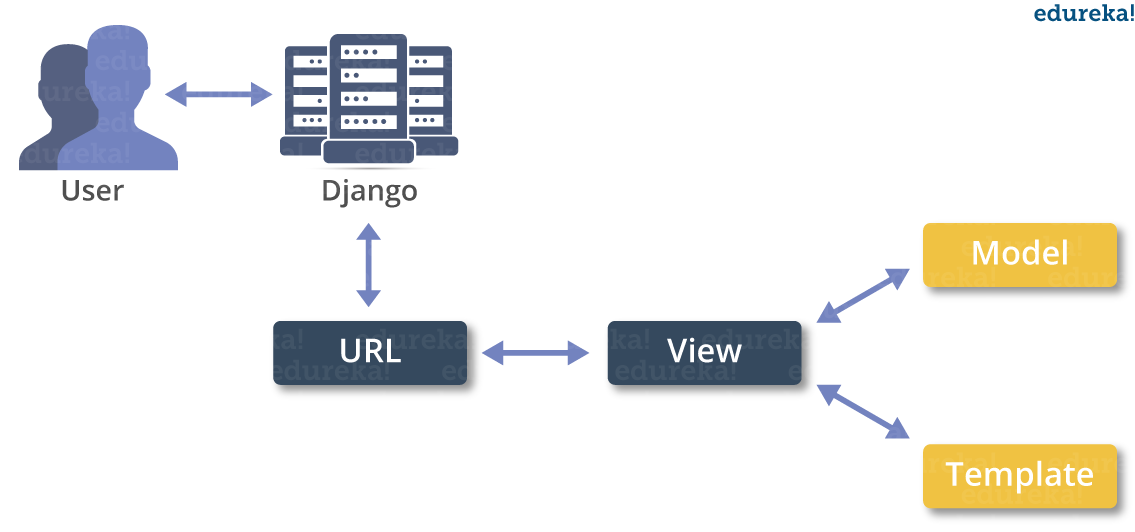
\includegraphics[width=15cm, height=6cm ]{images/ArchitectureDjango.png}
	\caption{Django Framework web architecture \cite{key26}}
	\label{django}
\end{figure} 

\begin{figure}[h]
	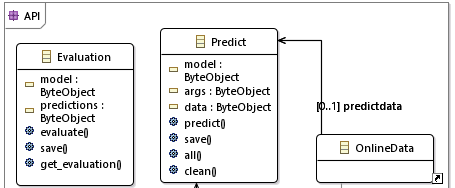
\includegraphics[ ]{images/APICD.png}
	\caption{Class diagram of our Ortho API }
	\label{ortho}
\end{figure} 

%\begin{figure}[h]
%	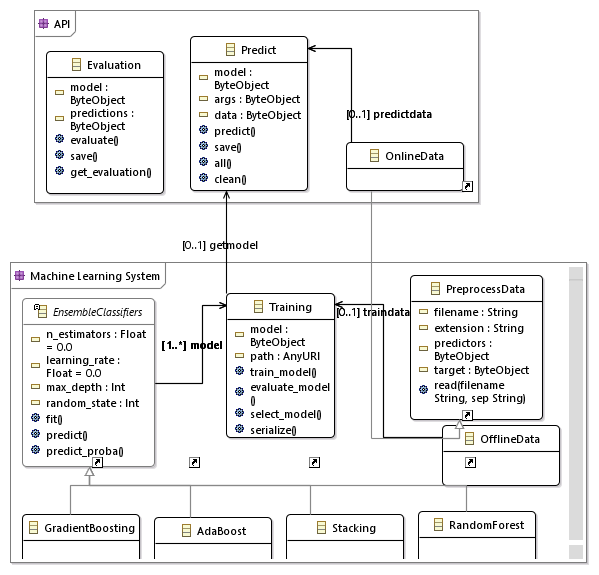
\includegraphics[ ]{images/ortho.png}
%	\caption{Connexion between our API and machine learning system }
%	\label{ortho}
%\end{figure} 

Notre API prend un formulaire web de Django en entrée et retourne un message de décision. Le framework django fait la validation du formulaire avant d'appeler l'API. Si tous les champs du formulaire sont bien validés et toutes les valeurs obligatoires sont présentes, alors l'API prend le formulaire et fait un pré-traitement des données. S'il trouve des données optionnelles qui sont vides ou nulles, il les remplace par ``\textbf{NaN}'' et s'il trouve des champs booléens, il les remplace par \textbf{0} si c'est \textbf{No} et par \textbf{1} si c'est \textbf{Yes}. \\

Le diagramme de classe présenté dans la figure \ref{ortho} permet de répondre à deux des cas d'utilisation que nous avons défini dans le diagramme de cas d'utilisation. Mais nous allons voir brièvement le fonctionnement de ce diagramme dans l'API:

\paragraph{Predict. } La classe qui répond à l'exigence \textbf{Predict} défini à l'introduction. Elle trois attributs et quatre méthodes. L'attribut \textbf{model} est le modèle machine learning désérialisé. L'attribut \textbf{args} est un dictionnaire qui stocke la décision rendue par le modèle et un message de prédiction. La méthode \textbf{predicit} calcule la prédiction en fonction des données du formulaire. La méthode \textbf{save} permet de sauvegarder les prédictions après avoir rendu une décision. 
\paragraph{Evaluation. } La classe d'évaluation permet de répondre à l'exigence \textbf{evaluate} défini dans le diagramme de cas d'utilisation à l'introduction générale. Elle contient deux attributs et trois méthodes. L'attribut \textbf{model} obtient le modèle du machine learning construit. L'attribut \textbf{predictions} est une liste de toutes les prédictions qui ont déjà traitées par le modèle. L'opération \textbf{evaluate} permet de d'évaluer le modèle en fonction de l'ensemble de \textbf{prédictions}. L'opération save sauvegarde le résultat de l'évaluation. \\


\begin{figure}[p]
	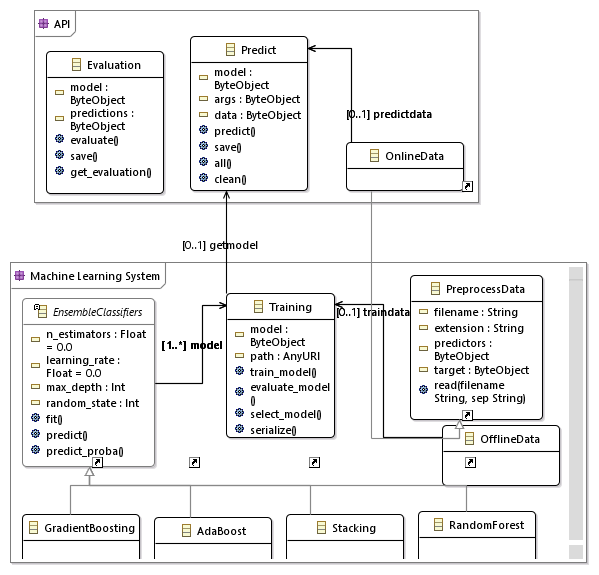
\includegraphics[ ]{images/ortho.png}
	\caption{Connexion between our API and machine learning system }
	\label{ortho}
\end{figure} 

%\section{Présentation de notre API}
%
%La table \ref{tab:api} nous présente les détails de notre API. La colonne "\textbf{Attribute or Method}" désigne les différents attributs et les méthodes que constitue notre API. et "\textbf{Comments}" dit ce que fait chaque attribut ou méthode. On précise aussi les différents paramètres de chaque fonction et leur valeur de retour. 
%
%\begin{table}[t]
%	\centering
%	\begin{tabular}{|p{6cm}|p{10cm}|}
%		\hline
%		\thead{Attribute or Method} & \thead{Comments}\\
%		\hline
%		 model & Variable that allows to recover model saved during the training phase  \\
%		 \hline
%		 preprocess\_request(form) & Method to prepare the data for transformation. Its loads the yaml file that contains the set of attributes wich are authorized and converts null values in NaN, Yes in 1 and No in 0. It returns a dcitionnary of attributes and values. \\
%		 \hline
%		 predict(form) & Function that allows prediction of new data. It takes a "form" input parameter and returns a decision message that says whether the patient should be fired or left. The "form" parameter is a django web form\\
%		 \hline
%		save\_prediction(form, y\_pred) & This function saves the new predictions in a database in order to analyze the behavior of the model in the future. It takes as input two parameters (form, y\_pred). The "form" parameter is always the same django form and "y\_pred" is the decision made by the model.\\
%		\hline
%		get\_predictions() & Returns all predictions\\
%		\hline
%	\end{tabular}
%	\caption{Presents details of our API}
%	\label{tab:api}
%\end{table}

La construction de l'API Ortho est un travail d'ingénierie de logiciels, ce qui permet de combiner ensemble deux champs d'études de l'informatique (\textbf{Machine learning et Software Engineering}) décrit dans la classe digramme présenté à la figure \ref{ortho}. Il faut relater que les modèles de machine learning ont besoin d'une couche d'ingénierie de logiciels pour leur rendre accessible aux utilisateurs qui ne comprennent rien en machine learning. Dans la vraie vie, ceux qui utilisent les modèles ne connaissent rien ni en machine learning ni en software engineering. C'est pourquoi dans tout lieu où il y a une équipe de data scientist qui travaillent, il y a aussi une équipe de développement de logiciels.

\newpage

\section{Déploiement de notre système}
Le système que nous développons a eu deux grandes phases de développement comme mentionné dans l'introduction. En plus, nous avons utilisé Django comme framework web qui a des fonctionnalités prédéfinies que nous utilisons dans notre projet. Maintenant nous allons montrer comment nous combinons tous ces morceaux ensemble pour donner un système. Le diagramme de déploiement présenté à la figure \ref{deployment} donne une vue générale des différentes connexions de chaque système. Voyons une brève description de chaque noeud de notre diagramme de déploiement:
\paragraph{Seattle University Data Server. } C'est le serveur de données de l'université Seattle. Ce serveur contient la base de données des patients qui ont subi des arthroplasties aux États-Unis. C'est notre source de données.
\paragraph{Machine Learning System. } C'est notre système ML que nous avons développé dans le chapitre 3. Il contient cinq composantes.
\paragraph{Web Repository. } C'est le dépôt web qui contient notre modèle machine learning.
\paragraph{Deployment System. } Le système de construction de notre API Ortho et l'environnement Django.
\paragraph{Server web. } L'hébergeur du site web Ortho predictions. Le service va être en ligne. 

\begin{figure}[h]
	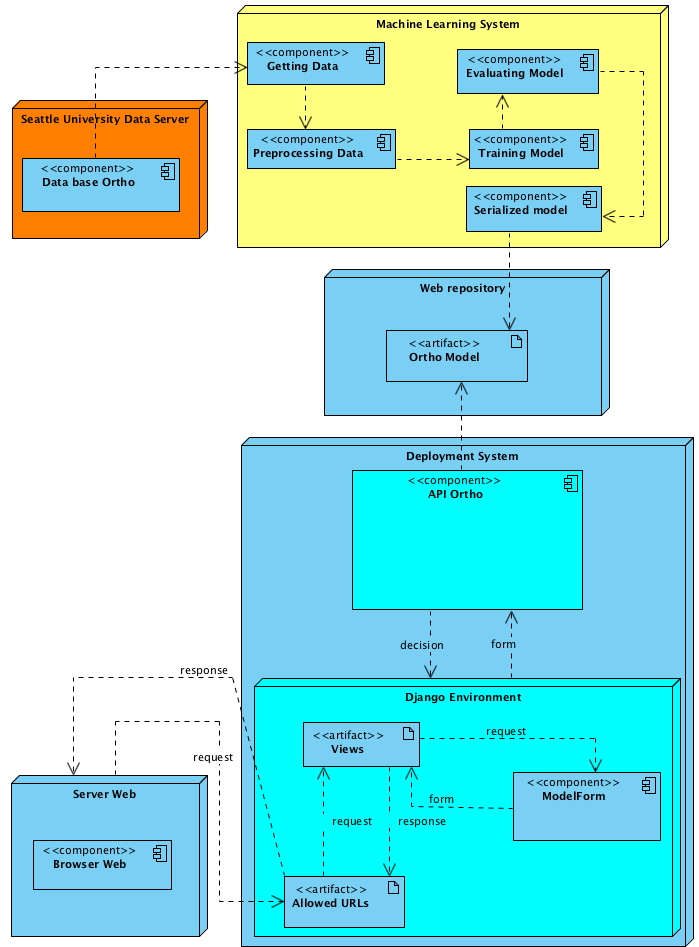
\includegraphics[width=17cm, height=24cm ]{images/deploymentdiag.png}
	\caption{A deployment diagram of our tool}
	\label{deployment}
\end{figure} 

%\newpage
%
%\section{Conclusion}
%Ce chapitre a détaillé tout ce que nous avons fait dans notre projet. C'est la phase de développement de notre projet. Nous avons vu la phase rapportant sur le développement d'un modèle d'apprentissage profond et la phase rapportant sur le génie de logiciel. La phase phase 1 permet la construction et la sérialisation du modèle  et la phase permet d'appliquer les techniques d'ingénierie de logiciel sur le modèle sérialisé.  Le chapitre qui suit va expliquer comment nous avons fait pour évaluer notre modèle de machine learning pour savoir s'il est fiable et répond aux critères d'évaluation escomptés.



\chapter{Évaluation}
\section{Évaluation du modèle machine learning}
L'évaluation des algorithmes d'apprentissage automatique est une partie essentielle de tout projet. Le modèle peut nous donner des résultats satisfaisants lorsqu'il est évalué à l'aide d'une métrique, par exemple \textbf{precision\_score}, mais il peut donner de mauvais résultats lorsqu'il est évalué par rapport à d'autres mesures, telles que \textbf{logarithmic\_loss} ou toute autre mesure de ce type. Évaluer un projet de machine learning est différent d'évaluer les projets de génie logiciels traditionnels. La différence est que pour évaluer de tels projets, il faut tenir compte des différentes théories de machine learning permettant de faire des évaluations sur des modèles. Ce que nous avons déjà dans la sous-section 2.3.1 portant sur la "\textbf{Mesure de performance des algorithmes de classification}" au chapitre "\textbf{Contexte théorique}". \\

Pour évaluer notre modèle, nous avons séparé notre ensemble de données en deux (Train Set et Test Set). Le train set a été utilisé pour construire le modèle et le test set pour faire l'évaluation du modèle. Nous avons séparé le jeu de données comme suit : 80\% pour le train set et 20\% pour le test set. Puisque notre jeu de données était déséquilibré, nous n'avons pas ré-échantillonné (resampling en anglais) notre ensemble de test, parce que les nouvelles données que le modèle va prédire se seront jamais ré-échantillonné. D'autres raisons de ce choix est que si nous ré-échantillonnons l'ensemble de test, il est fort probable que le modèle soit biaisé, ce qui provoquera de fausses prédictions. \\

  \begin{table}[h]
	\centering
	\begin{tabular}{|p{6cm}|p{10cm}|}
		\hline
		 \thead{Model's name} & AdaBoostClassifier\\
		\hline
		  \thead{Precision score} & 0.9291845493562232 \\
		 \hline
		  \thead{Recall score} & 0.9002079002079002\\
		 \hline
		  \thead{Area under Curve} & 0.8511029411764706 \\ 
		 \hline
		  \thead{F1 score} & 0.914466737064414\\
		\hline
	\end{tabular}
	\caption{Gives different results of our model evaluation}
	\label{tab:eval}
\end{table}

La table \ref{tab:eval} donne les résultats de l'évaluation de notre modèle sélectionné comme le meilleur. On pourrait constater que cette table est ressemblée à la table de comparaison des différents algorithmes entrainés dans le projet (table \ref{tab:ensemble}). La raison est que pour comparer et sélectionner les différents algorithmes, il faut d'abord évaluer chaque algorithme. C'est comme une évaluation anticipée. Une interprétation sommaire de cette évaluation est que 8\% des prédictions faites par le modèle est erroné et 92\% sont correctement classées. Pour faire cette interpretation, nous nous tenons compte du '' \textbf{Precision score} '' de la table \ref{tab:eval}. 

\section{Evaluation de notre API Ortho}
Pour évaluer notre API, nous avons construit un diagramme de séquence qui montre comment les orthopédistes peuvent utiliser l'API pour prédire un retour. Et l'API à son tour se connecte au repository du machine learning pour charger le modèle sérialisé par le système machine learning. La figure \ref{SequenceDiag} est la classe diagramme qui montre les interactions entre les orthopédistes et ses différents objets impliqués dans le scénario de la prédiction.

Nous allons décrire brièvement les différents messages qui permettent à un orthopédiste de réussir une prédiction.
\begin{enumerate}
\item \textbf{Fill form and press predict.} Quand l'orthopédiste accède à la page de la prédiction, il doit remplir le formulaire et ensuite appuyer sur le bouton Predict pour envoyer le formulaire;
\item \textbf{Validate Form.} Le moteur Django est engagé de faire la validation automatique du formulaire selon les critères qu'on avait précisés dans l'étape de conception du formulaire;
\item \textbf{Form is validated.} Si le formulaire est validé, Django retourne un message que la validation est vraie c'est-à-dire le formulaire est bien rempli;
\item \textbf{Predict decision using the validated form.} Le formulaire rempli est passé à l'API comme paramètre. L'API fait le traitement du formulaire tel que nous avons vu dans la phase de construction de l'API.
\item \textbf{Load model.} L'API charge le modèle qui est hébergé dans le repository de machine learning. Le repository peut être le serveur de la compagnie ou le cloud;
\item \textbf{Model loaded.} L'API utilise le modèle pour faire la prédiction utilisant le formulaire pré-traité et rendu sous forme d'un dataframe (un objet de la classe DataFrame de la librairie Pandas);
\item \textbf{Decision predicted.} L'API rend la décision si le patient doit retourner ou rester à l'hôpital;
\item \textbf{A message with the decision.} Une réponse en format de chaine de caractère est rendu à l'utilisateur dans ce cas l'orthopédiste. Cette réponse est le message de la décision.
\end{enumerate}


 
\begin{figure}[p]
	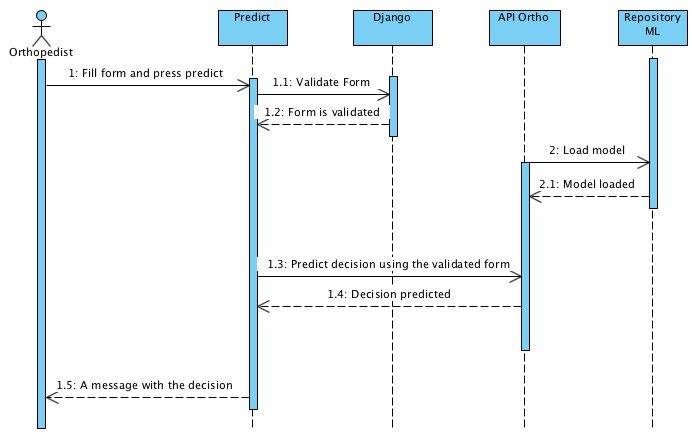
\includegraphics[width=17cm, height=10cm ]{images/SequenceDiag.png}
	\caption{Sequence diagram for evaluating our API tool}
	\label{SequenceDiag}
\end{figure} 

\section{Limitations et travaux futurs}
Notre projet est loin d'être exhaustif, il reste beaucoup de choses à faire mais les parties essentielles du projet sont réalisées. Nous pouvons considérer tout ce que nous avons fait jusqu'à présent dans ce projet comme étant une première version du système. Pour le moment, on peut utiliser le système pour faire la prédiction et l'évaluation de notre modèle déployé. C'est-à-dire n'importe quel orthopédiste peut utiliser le système pour prédire si son patient doit rester à l'hôpital et s'il doit retourner chez lui après une arthroplastie. Pour que le médecin orthopédiste puisse faire ces prédictions, il doit, préalablement remplir un formulaire web qui contient les champs nécessaires pour compléter un dossier médical.   \\

Comme travaux futurs, nous prévoyons inclure les modules qui gèrent le monitoring et management du modèle. Et aussi la gestion des sessions puisque tout le monde peut avoir accès au module de prédictions mais les modules monitoring et management sont réservés aux administrateurs du système.    
\newpage

\chapter{Travaux connexes}
Nous n'avons pas trouvé de travaux connexes directement liés à notre domaine c'est-à-dire aucun organisme n'a encore développé de systèmes liés au risque de retour des patients après une arthroplastie. Par contre nous avons trouvé des projets qui ont des points similaires par rapport à notre projet tels que les classes déséquilibrées, la technique SMOTE, le problème de classification et les algorithmes ensemblistes. Aussi nous avons trouvé des APIs conçus pour être utilisés dans l'apprentissage automatique.\\

MLlib, une bibliothèque d'apprentissage automatique distribuée de Apache Spark (plateforme populaire adaptée aux tâches d'apprentissage machine itératives) a été présenté par Xiangrui Meng et al. \cite{key34}. La bibliothèque cible les paramètres d'apprentissage à grande échelle qui bénéficient du parallélisme des données ou du parallélisme des modèles pour stocker et exploiter des données ou des modèles. MLlib consiste en des implémentations rapides et évolutives d'algorithmes d'apprentissage standard pour les paramètres d'apprentissage communs, y compris la classification, la régression, le filtrage collaboratif, la mise en grappe et la réduction de la dimensionnalité. Il fournit également une variété de statistiques sous-jacentes, d'algèbre linéaire et de primitives d'optimisation. Écrit dans Scala et utilisant des bibliothèques d'algèbre linéaire (basées sur C ++) sur chaque nœud, MLlib inclut des API Java, Scala et Python, et est publié dans le cadre du projet Spark sous la licence Apache 2.0. MLlib  fournit une API de haut niveau qui exploite l'écosystème riche de Spark pour simplifier le développement de pipelines d'apprentissage automatique de bout en bout. Dans notre projet, nous avons conçu notre propre API spécifique à nos besoins. \\

MXNet est une bibliothèque d'apprentissage automatique multi-langages pour faciliter le développement d'algorithmes ML, en particulier pour les réseaux neuronaux profonds. Incorporé dans le langage hôte, il mélange l'expression symbolique déclarative avec le calcul tensoriel impératif pour maximiser l'efficacité et la flexibilité. Il offre une différenciation automatique pour dériver des dégradés. MXNet est efficace en termes de calcul et de mémoire et fonctionne sur divers systèmes hétérogènes, allant des périphériques mobiles aux clusters GPU distribués. La conception de l'API et l'implémentation du système de MXNet ont été réalisés par Tianqi Chen et al. \cite{key35}. Nous avons préféré de développer notre propre API en fonction de nos besoins et notre ensemble de données. En machine learning, il n'y a pas d'API meilleur que d'autres, tout dépend du contexte de développement qu'on se trouve et la situation à laquelle on fait face. Souvent, il vaut mieux de développer ses propres outils spécifiques et adaptés à ce qu'on veut faire. \\

Une étude a été réalisée par Lars Buitinck et al. \cite{key36} sur l'API scikit-learn et de la manière dont elle mappe les concepts et les tâches d'apprentissage automatique sur les objets et les opérations dans le langage de programmation Python. Ils ont montré comment une API cohérente à travers le paquet rend scikit-learn très utile dans la pratique: expérimenter avec différents algorithmes d'apprentissage est aussi simple que de substituer une nouvelle définition de classe. Grâce à des interfaces de composition telles que Pipelines, Feature Unions et méta-estimateurs, ces blocs de construction simples conduisent à une API puissante et capable d'accomplir une grande variété de tâches d'apprentissage dans une petite quantité de code facile à lire. Par le biais du typage de canard, l'API cohérente conduit à une bibliothèque qui est facilement extensible, et permet aux estimateurs définis par l'utilisateur d'être incorporés dans le flux de travail scikit-learn sans héritage d'objet explicite. Notre API est aussi connecté à l'API  scikit-learn pour donner de bons résultats dans notre projet. Par exemple, notre API doit accéder à notre modèle de machine learning conçu en utilisant les algorithmes classificateurs de la librairie  scikit-learn. Cette techinque produit de bons résultats puisque l'API  scikit-learn a été conçu pour être utilisé de cette manière.\\

Alberto Fernández et al. \cite{key30} ont fourni une analyse expérimentale approfondie qui permettra de déterminer le comportement des différentes approches proposées dans la littérature spécialisée. Tout d'abord, ils ont utilisé des schémas de binarisation, c'est-à-dire, un par rapport à un et un par rapport à tous, afin d'appliquer les approches standard à la résolution de problèmes de classes binaires déséquilibrées. Deuxièmement, ils ont appliqué plusieurs procédures ad hoc qui ont été conçues pour le scénario d'ensembles de données déséquilibrés avec plusieurs classes. Leur étude expérimentale inclut plusieurs algorithmes bien connus de la littérature tels que les arbres de décision, les machines à vecteurs de support et l'apprentissage par instance, avec l'intention d'obtenir des conclusions globales à partir de différents paradigmes de classification. Tandis que dans notre projet nous avons utilisé les algorithmes ensemblistes qui donnent de meilleurs résultats que les algorithmes simples utilisés dans cette étude.\\

Sreejita Ghosh et al.  \cite{key31} ont réalisé un travail dans le domaine biomédical, un taux de détection élevé de maladies éventuellement rares est généralement hautement souhaitable alors que des erreurs dans la classe majoritaire (par exemple des témoins sains) peuvent être plus acceptables. Par conséquent, l'optimisation de la précision prédictive globale est souvent inadaptée. Ils ont analysé un grand ensemble de données de GC / MS urinaires de 829 contrôles et 68 patients souffrant de l'un des trois troubles stéroïdiens innés. Ils ont utilisé 2 algorithmes comparables capables de gérer de grandes quantités de données manquantes. En outre, ils ont comparé différentes stratégies pour traiter les données fortement déséquilibrées, y compris le sous-échantillonnage, le sur-échantillonnage et l'introduction de coûts par classe. Dans cette étude, ils ont utilisé SMOTE pour équilibrer mais ils n'ont pas utilisé les algorithmes ensemblistes qui sont conçus pour être adaptés aux jeux de données déséquilibrés. \\

Rukshan Batuwita and Vasile Palade \cite{key32} ont démontré que les SVM (Support Vector Machines) pourraient produire des résultats sous-optimaux avec des jeux de données déséquilibrés, malgré c'est une technique d'apprentissage automatique très populaire. Autrement dit, un classificateur SVM formé sur un ensemble de données déséquilibré peut produire des modèles sous-optimaux qui sont biaisés vers la classe majoritaire et ont une faible performance sur la classe minoritaire, comme la plupart des autres paradigmes de classification. Diverses techniques de pré-traitement et d'algorithmique des données ont été proposées dans la littérature pour atténuer ce problème pour les SVM. Il existe des méthodes qui ont utilisé la combinaison des deux méthodes externes et internes pour résoudre le problème de déséquilibre de classe pour les SVM. La méthode hybride de l'ensemble des machines à noyau (HKME) combine un SVM binaire standard et un classificateur SVM à une classe pour résoudre le problème du déséquilibre de classes. La différence avec notre projet, c'est que nous avons utilisé des techniques dédiées pour faire le resampling, non pas des techniques combinées comme proposé dans cet article.\\

Rok Blagus and Lara Lusa \cite{key33}  ont appliqué SMOTE (Synthetic Minority Oversampling TEchnique ) à des données déséquilibrées de classe à haute dimension (à la fois simulées et réelles) et ont également utilisé des résultats théoriques pour expliquer le comportement de SMOTE. Les principales conclusions de leur analyse sont:

\begin{itemize}
\item dans le réglage de faible dimension SMOTE est efficace pour réduire le problème de déséquilibre de classe pour la plupart des classificateurs;

\item SMOTE n'a pratiquement aucun effet sur la plupart des classificateurs formés aux données de grande dimension;

\item lorsque les données sont de haute dimension SMOTE est bénéfique pour les classificateurs k-NN si la sélection de variables est effectuée avant SMOTE;

\item SMOTE n'est pas bénéfique pour les classificateurs d'analyse discriminante, même dans le cadre de basse dimension;

\item sous-échantillonnage ou, pour certains classificateurs, l'ajustement de coupure est préférable à SMOTE pour les tâches de prédiction de classe de grande dimension.

\end{itemize}

Dans cette étude, les auteurs ont décrit les avantages d'utiliser SMOTE mais ils n'ont pas proposé les algorithmes qui fonctionnent mieux avec cette technique. Si vous utilisez SMOTE dans vos projets, vous ne pouvez pas utiliser les algorithmes classiques de machine learning parce que les résultas peuvent être biaisés facilement. Il faut toujours utilisé les classificateurs fort comme les ensemblistes.


  

%Philip K. Chan, Computer Science, Florida Institute of Technology \& Salvatore J. Stolfo, Department of Computer Science, Columbia University \cite{key23} ont travaillé sur un projet de détection de fraude par carte de crédit. Ils ont eu leur dataset déséquilibrés (distributions uniformes dans leur article), 20\% de cas étaient frauduleux contre 80\% non-frauduleux.  Pour rappel, la distribution de notre dataset est présentée à la table \ref{tab:target}, avec 11\% de classes négatives et 89\% de classe positives. Les auteurs ont utilisés juste un  algorithme stacking comme méthodes d'ensemble, tandis que nous, nous avons essayé quatre types d'algorithmes différents en vue de sélectionner le meilleur. Pour le resample(ré-échantillonnage), ils ont utilisé le random over-sampling comme méthode, cette méthode est trop basique pour ces genres de situation car elle ne permet pas de gérer le overfitting. Tandis que nous, nous avons opté pour la technique de boosting qui a beaucoup plus d'avantage, car elle permet de gérer la variance et le biais.\\
%
%Yuchun Tang et al. \cite{key29} ont travaillé sur un projet de detection d'emails spam et ceux qui sont non-spam. Dans leur projet, le dataset est hautement déséquilibré comme montré à la table \ref{tab:Tang}. C'est plus déséquilibré que notre dataset. Il est courant que dans n'importe quel serveur web que les emails spam sont hautement plus nombreux que ceux qui sont non-spam. Ce qui provoque un déséquilibre sérieux dans l'ensemble de données. \\
%
%\begin{table}[h]
%	\centering
%	\begin{tabular}{| p{5cm} |p{2cm} |  p{2cm}|}
%		\hline
%		 & \thead{spam} & \thead{non-spam} \\
%		\hline
%		  training data & 93.96\% & 6.04\% \\
%		 \hline
%		  validation data & 93.09\% & 6.91\% \\
%		 \hline
%		 testing data & 94.99\% & 5.01\%  \\ 
%		 \hline
%	\end{tabular}
%	\caption{Target value of Yuchun Tang et al. project}
%	\label{tab:Tang}
%\end{table}
%
%Comme technique de resampling, le \textbf{Granular Computing} et le \textbf{SVM (\textit{Support Vector Machines})} sont utilisés pour le sous-échantillonnage  (\textbf{\textit{under-sampling en anglais}}) en conservant des échantillons informatifs tout en éliminant les échantillons non pertinents, redondants ou même bruyants. Après le sous-échantillonnage, les données sont nettoyées et, par conséquent, un bon classificateur peut être modélisé pour la classification IP en termes d'efficacité et d'efficience. La technique utilisée dans ce projet a une désavantage très importante, c'est la perte d'informations. Il faut être prudent quand on utilise cette technique, puisqu'on peut perdre des informations pertinentes pour l'entraînement du modèle. Comme précisé dans leur article, les informations supprimées sont non-pertinentes pour le projet; mais généralement, c'est une technique à éviter ou à utiliser minutieusement. \\
%
%Comme algorithmes de classification, ils ont utilisés les quatre algorithmes suivants  \cite{key29}:
%\begin{enumerate}
%\item GSVM-BA algorithm for building a decision tree
%\item The NBTree algorithm for building a decision tree with naïve Bayes classifiers at the leaves
%\item The Logistic algorithm for building a multinomial logistic regression model with a ridge estimator
%\item The SVM algorithm for building a support vector machine
%\end{enumerate}
%
%Le meilleur algorithme obtenu après évaluation était GSVM-BA, avec le score 83\%  \cite{key29}. Tandis que dans notre projet, nous avons obtenu  92\% avec l'algorithme AdaBoostClassifier qui est un algorithme de boosting qui donne de meilleurs résultats que n'importe quel autre algorithme. Puisque ce projet a été développé depuis 2008, c'est sûr à cette époque on ne parlait pas encore des algorithmes de méthodes d'ensemble. \\
%
%Pour conclure le chapitre sur les travaux connexes, nous répétons ce que nous avons dit au commencement de ce chapitre qu'il n'y a pas de projets déjà réalisés sur l'évaluation du risque de retour. Mais comme notre dataset était déséquilibré, nous avons comparé notre projet avec deux autres projets qui ont eu, eux-aussi, leurs datasets déséquilibrés. Nous avons vu les différentes techniques de resampling et les différents algorithmes que les auteurs ont utilisés dans le cadre de leurs projets. Finalement, nous avons comparé leurs techniques avec les nôtres, aussi les différents résultats obtenus après évaluation.  



\newpage

\chapter{Conclusion générale}

Nous avons développé un outil qui permet aux orthopédistes américains de déterminer de façon automatique quand un patient doit retourner chez lui après une arthroplastie et quand il doit reste à l'hôpital pour une réadaptation. Le projet était important parce que les compagnies d'assurance de santé américaine ne couvrent pas les frais relatifs à la réadaptation d'un patient qui sont très élevés soit environ \$ 30,000 par réadaptation. Ces coûts doivent être couverts par les hôpitaux et le compagnies d'assurance ne couvrent que les arthroplasties qui sont les opérations. Nous avons dit également, il est très fastidieux pour un médecin de vérifier manuellement un dossier patient compte tenu du volume des informations. Grâce à notre outil les docteurs orthopédistes américains peuvent prédire automatiquement la décision à prendre après une arthroplastie.  \\    

Pour développer cet outil, nous avons démontré comment nous pouvons combiner les techniques de machine learning et celles du software engineering pour aboutir à l'implémentation d'un système complet. Par conséquent, notre projet a été divisé en deux grandes phases qui, elles-mêmes, contiennent plusieurs étapes. Dans la première phase du projet, on a réalisé le cycle de travail complet d'un data scientist depuis l'obtention des données jusqu'à la modélisation (étape qui consiste à entrainer différents modèles machine learning en vue  de sélectionner le meilleur qui répond à notre problématique). Cette phase se termine par la sérialisation du modèle estimé meilleur en vue de son utilisation future. Dans la deuxième phase, nous avons vu le déploiement de notre modèle machine learning sérialisé. Cette phase est la conception de notre API Ortho. Ce dernier a été conçu en utilisant le framework web Django que nous avons décrit dans le chapitre 4. \\

Pour chaque phase de notre projet, nous avons construit un diagramme de cas d'utilisation expliquant les différentes exigences que notre système doit satisfaire et nous avons donné une brève explication de chaque cas d'utilisation dans l'introduction générale. Dans les chapitres 3 et 4 nous avons dessiné deux diagrammes de classe, un pour chaque diagramme de cas d'utilisation dans le but d'expliquer les différentes opérations nécessaires pouvant satisfaire les exigences que nous avons décrites. Nous avons vu un diagramme de déploiement permettant de connecter les différents noeuds facilitant le déploiement du système. 

\paragraph{Difficultés rencontrées. } 
Les développements des projets de machine learning peuvent avoir des problèmes différents  l'un de l'autre. Les facteurs qui déclenchent ces problèmes peuvent être liées soit au développement technique du projet, soit à l'administration ou aux interdictions légales. Pour réaliser ce projet de stage, nous n'étions pas exempts de ce problème, nous avons fait face à des difficultés techniques et parfois même administratives comme tout autre projet dans un sens général. La liste suivante donne une vue générale de quelques-unes que nous avons rencontrées :
\begin{itemize}
\item La première difficulté que nous avons eu c'est de combiner le machine learning et le software engineering. Puisqu'au début du stage je n'ai pas eu de connaissances en machine learning;
\item choisir la meilleure technique de ré-échantillonnage (resampling) est une difficulté car aucune technique n'est supérieure à d'autres, tout dépend de la problématique étudiée. Pour choisir le SMOTE, il a fallu qu'on essaye plusieurs techniques et comparer les résultats pour déterminer le meilleur en fonction de notre jeu de données;
\item le choix de l'algorithme était une autre difficulté puisque les algorithmes traditionnels ne fonctionnent pas sur un jeu de données déséquilibré. Même pour choisir un algorithme ensembliste est difficile car chacun a une approche différente l'une de l'autre. Par exemple les algorithmes boosting sont séquentiels tandis que les bagging sont avec remplacement. Donc le choix devient difficile;
\item l'ensemble de données était très petit pour faire l'entraînement des modèles. En machine learning plus votre ensemble de données est petit, plus votre modèle n'est pas fiable. Trouver de nouvelles données est difficile puisque ça doit prendre six mois environ à cause des démarches administratives à entreprendre;
\item les données médicales sont des données très sensibles. Avoir accès à ces données est difficile car c'est interdit par la loi.  
\end{itemize}

\paragraph{Leçons apprises. } 
Puisque nous soutenons que nous avons rencontré des problèmes dans le développement de notre projet, il est primordial de faire ressortir les différentes leçons que nous avons apprises à partir de ces difficultés. Voici deux grandes leçons que j'ai apprises au cours du développement de ce projet : 

\begin{itemize}
\item \textbf{Combinaison de plusieurs spécialités.} Nous avons appris que toutes les spécialités informatiques peuvent se combiner les unes avec les autres. Par exemple un API développé en Software engineering peut être utilisé pour connecter à des modèles développés en machine learning. On peut aussi utiliser les diagrammes UML pour décrire un système de machine learning ou n'importe quel autre système en général. De même que les sciences ne sont pas isolées entre elles, de même aussi les spécialités informatiques ne sont pas isolées entre elles;
\item \textbf{Technologies apprises.}  Au début de ce projet, nous ne savions rien ni en machine learning ni en python. Maintenant nous savons utiliser toutes les librairies de machine learning de python telles que sckit-learn, mlxtend, pandas, matplotlib, numpy, scipy etc. Nous avons appris à développer en Django un framework web de python dont nous avons utilisé pour le développement de notre API. 
\end{itemize}

Notre outil va être déployé sur le serveur web de la compagnie pour laquelle je fais le stage (ML+). L'outil va être en ligne et son utilisation sera gratuite pour tous les orthopédistes américains qui veulent uniquement prédire un retour. Mais ceux qui veulent veulent évaluer, suivre et gérer un modèle doivent être d'abord administrateur du système. Pour être administrateur, il faut contacter de ML+ et vous aurez un compte qui vous donnera accès; néanmoins certaines conditions peuvent être appliquées tel que un frais unique. Le code de source de notre projet est disponible sur Github et le lien pour y accéder est le suivant : https://github.com/top1986/NewIntershipProject.   


\newpage

\appendix
\chapter{Annexe A}

%\begin{figure}[h]
%	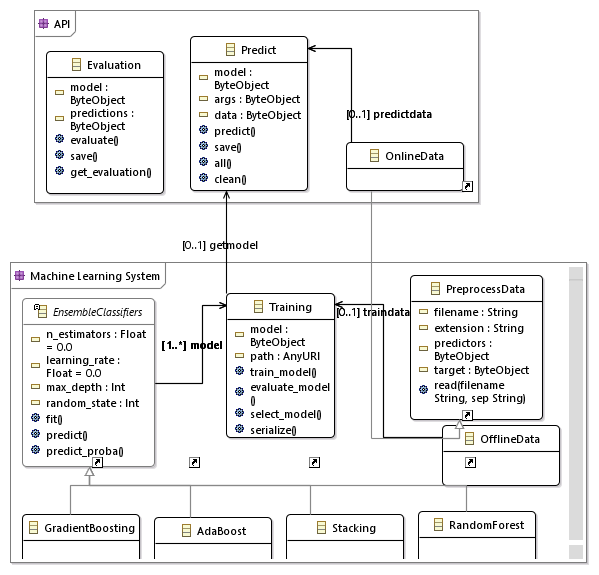
\includegraphics[ ]{images/ortho.png}
%	\caption{A class diagram to explain connexion between our API and machine learning system }
%	\label{cd}
%\end{figure} 




\begin{longtable}{ | p{.25\textwidth} | p{.15\textwidth} | p{.10\textwidth}  | p{.10\textwidth} | p{.40\textwidth} |  } 
\hline
\textbf{Feature name} & \textbf{datatype} & \textbf{non-null }& \textbf{ null } & \textbf{Comments}\\ \hline

Side & Categorical & 2718 & 0 & Détermine si c'est à gauche ou à droite du patient a eu son arthroplastie. Deux valeurs possibles : R (pour Right en anglais) et  L (Pour Left en anglais) \\ \hline 
Procedure & Boolean & 2718 & 0& On veut savoir si oui ou non le patient a eu une procédure dans le passé \\ \hline 
RawDx & Categorical & 2718 & 0 & Diagnostique brute du patient  \\ \hline 
PriorContralateral & Boolean & 2703 & 15& On veut savoir si oui ou non le patient est atteint de \textit{PriorContralateral} \\ \hline 
TSA & Boolean & 2718 & 0& On veut savoir si oui ou non le patient est atteint de \textit{TSA} \\ \hline 
RTSA & Boolean & 2718 & 0& On veut savoir si oui ou non le patient est atteint de \textit{RTSA} \\ \hline 
Tendon Transfer & Boolean & 2718 & 0& On veut savoir si oui ou non le patient est atteint de \textit{Tendon Transfer} \\ \hline 
Dx1 & Categorical & 2718 & 0 & Représente diagnostique 1 \\ \hline 
Dx2 & Categorical & 176 & 2542 & Représente diagnostique 2 \\ \hline 
Dx3 & Categorical & 2 & 2716 & Représente diagnostique 3 \\ \hline 
GHOA & Boolean & 2718 & 0& On veut savoir si oui ou non le patient est atteint de \textit{GHOA} \\ \hline 
AVN & Boolean & 2718 & 0& On veut savoir si oui ou non le patient est atteint de \textit{AVN} \\ \hline 
RCT & Boolean & 2718 & 0& On veut savoir si oui ou non le patient est atteint de \textit{RCT} \\ \hline 
FailedRCR & Boolean & 2718 & 0& On veut savoir si oui ou non le patient est atteint de \textit{FailedRCR} \\ \hline 
ComboRCT & Boolean & 2718 & 0& On veut savoir si oui ou non le patient est atteint de \textit{ComboRCT} \\ \hline 
RCTA & Boolean & 2718 & 0& On veut savoir si oui ou non le patient est atteint de \textit{RCTA} \\ \hline 
IA & Boolean & 2718 & 0& On veut savoir si oui ou non le patient est atteint de \textit{IA} \\ \hline 
PTA & Boolean & 2718 & 0& On veut savoir si oui ou non le patient est atteint de \textit{PTA} \\ \hline 
PHFx & Boolean & 2718 & 0& On veut savoir si oui ou non le patient est atteint de \textit{PHFx} \\ \hline 
PHFxSequelae & Boolean & 2718 & 0& On veut savoir si oui ou non le patient est atteint de \textit{PHFxSequelae} \\ \hline 
Other & Boolean & 2718 & 0& On veut savoir si oui ou non le patient est atteint de \textit{Other} \\ \hline 
AGE\_AT\_ADMIT & Numerical & 2718 & 0 & L'âge du patient \\ \hline 
ASA\_SCORE & Numerical & 2716 & 2 & Les commentaires sont à venir \\ \hline 
Gender & Boolean & 2718 & 0& On veut savoir si oui ou non le patient est un \textit{Gender} \\ \hline 
Female & Boolean & 2718 & 0& On veut savoir si oui ou non le patient est un \textit{Female} \\ \hline 
Discharge & Boolean & 2718 & 0& On veut savoir si oui ou non le patient doit retourner chez lui \\ \hline 
Height & Numerical & 2293 & 425 & La hauteur du patient \\ \hline 
Weight & Numerical & 2301 & 417 & Le poids du patient \\ \hline 
BMI & Numerical & 2283 & 435 & L'indice de masse corporelle (IMC)- BMI en anglais \\ \hline 
PreOpHgb & Numerical & 272 & 2446 & Hémoglobines blanches du patient \\ \hline 
PreOpCr & Numerical & 255 & 2463 & Conditions pré-opératoires du patient \\ \hline 
PreOpALC & Numerical & 157 & 2561 &  Conditions pré-opératoires du patient \\ \hline 
PreOpGlucose & Numerical & 253 & 2465 & Glucose du patient \\ \hline 
arrhythmias & Boolean & 2092 & 626& On veut savoir si oui ou non le patient est atteint de \textit{arrhythmias} \\ \hline 
valvular & Boolean & 2092 & 626& On veut savoir si oui ou non le patient est atteint de \textit{valvular} \\ \hline 
pulm circ & Boolean & 2092 & 626& On veut savoir si oui ou non le patient est atteint de \textit{pulm circ} \\ \hline 
PVD & Boolean & 2092 & 626& On veut savoir si oui ou non le patient est atteint de \textit{PVD} \\ \hline 
HTNw/oCx & Boolean & 2092 & 626& On veut savoir si oui ou non le patient est atteint de \textit{HTNw/oCx} \\ \hline 
HTNw/Cx & Boolean & 2092 & 626& On veut savoir si oui ou non le patient est atteint de \textit{HTNw/Cx} \\ \hline 
Paralysis & Boolean & 2092 & 626& On veut savoir si oui ou non le patient est atteint de \textit{Paralysis} \\ \hline 
other neuro & Boolean & 2092 & 626& On veut savoir si oui ou non le patient est atteint de \textit{other neuro} \\ \hline 
chronic pulm & Boolean & 2092 & 626& On veut savoir si oui ou non le patient est atteint de \textit{chronic pulm} \\ \hline 
DMw/oCx & Boolean & 2092 & 626& On veut savoir si oui ou non le patient est atteint de \textit{DMw/oCx} \\ \hline 
DMw/Cx & Boolean & 2092 & 626& On veut savoir si oui ou non le patient est atteint de \textit{DMw/Cx} \\ \hline 
hypothyroid & Boolean & 2092 & 626& On veut savoir si oui ou non le patient est atteint de \textit{hypothyroid} \\ \hline 
renal failure & Boolean & 2092 & 626& On veut savoir si oui ou non le patient est atteint de \textit{renal failure} \\ \hline 
liver failure & Boolean & 2092 & 626& On veut savoir si oui ou non le patient est atteint de \textit{liver failure} \\ \hline 
PUD & Boolean & 2092 & 626& On veut savoir si oui ou non le patient est atteint de \textit{PUD} \\ \hline 
AIDS & Boolean & 2092 & 626& On veut savoir si oui ou non le patient est atteint de \textit{AIDS} \\ \hline 
L0oma & Boolean & 2092 & 626& On veut savoir si oui ou non le patient est atteint de \textit{L0oma} \\ \hline 
Mets & Boolean & 2092 & 626& On veut savoir si oui ou non le patient est atteint de \textit{Mets} \\ \hline 
solidCaw/oMets & Boolean & 2092 & 626& On veut savoir si oui ou non le patient est atteint de \textit{solidCaw/oMets} \\ \hline 
RA/CVD & Boolean & 2092 & 626& On veut savoir si oui ou non le patient est atteint de \textit{RA/CVD} \\ \hline 
coagulopathy & Boolean & 2092 & 626& On veut savoir si oui ou non le patient est atteint de \textit{coagulopathy} \\ \hline 
obesity & Boolean & 2092 & 626& On veut savoir si oui ou non le patient est atteint de \textit{obesity} \\ \hline 
weightLoss & Boolean & 2092 & 626& On veut savoir si oui ou non le patient est atteint de \textit{weightLoss} \\ \hline 
fluidElectrolyte & Boolean & 2092 & 626& On veut savoir si oui ou non le patient est atteint de \textit{fluidElectrolyte} \\ \hline 
bloodLossAnemia & Boolean & 2092 & 626& On veut savoir si oui ou non le patient est atteint de \textit{bloodLossAnemia} \\ \hline 
DeficiencyAnemia & Boolean & 2092 & 626& On veut savoir si oui ou non le patient est atteint de \textit{DeficiencyAnemia} \\ \hline 
EtOH & Boolean & 2092 & 626& On veut savoir si oui ou non le patient est atteint de \textit{EtOH} \\ \hline 
Drugs & Boolean & 2092 & 626& On veut savoir si oui ou non le patient est atteint de \textit{Drugs} \\ \hline 
Psychosis & Boolean & 2092 & 626& On veut savoir si oui ou non le patient est atteint de \textit{Psychosis} \\ \hline 
Depression & Boolean & 2092 & 626& On veut savoir si oui ou non le patient est atteint de \textit{Depression} \\ \hline 
Plavix & Numerical & 2482 & 236 & Les commentaires sont à venir \\ \hline 
Dabigatran & Boolean & 2482 & 236& On veut savoir si oui ou non le patient est atteint de \textit{Dabigatran} \\ \hline 
Enoxaparin & Numerical & 2482 & 236 & Les commentaires sont à venir \\ \hline 
Rivaroxaban & Numerical & 2482 & 236 & Les commentaires sont à venir \\ \hline 
Warfarin & Numerical & 2482 & 236 & Les commentaires sont à venir \\ \hline 
PreOpNarcotic & Boolean & 900 & 1818& On veut savoir si oui ou non le patient est atteint de \textit{PreOpNarcotic} \\ \hline 
PreOpBloodThinner & Boolean & 900 & 1818& On veut savoir si oui ou non le patient est atteint de \textit{PreOpBloodThinner} \\ \hline 
PreOpSteroids & Boolean & 900 & 1818& On veut savoir si oui ou non le patient est atteint de \textit{PreOpSteroids} \\ \hline 
PreOpInsulin & Boolean & 900 & 1818& On veut savoir si oui ou non le patient est atteint de \textit{PreOpInsulin} \\ \hline 
PreOpDMMeds & Boolean & 900 & 1818& On veut savoir si oui ou non le patient est atteint de \textit{PreOpDMMeds} \\ \hline 
Oxycodone & Boolean & 900 & 1818& On veut savoir si oui ou non le patient est atteint de \textit{Oxycodone} \\ \hline 
Hydrocodone & Boolean & 900 & 1818& On veut savoir si oui ou non le patient est atteint de \textit{Hydrocodone} \\ \hline 
Vicodin & Boolean & 900 & 1818& On veut savoir si oui ou non le patient est atteint de \textit{Vicodin} \\ \hline 
percocet & Boolean & 900 & 1818& On veut savoir si oui ou non le patient est atteint de \textit{percocet} \\ \hline 
Oxycontin & Boolean & 900 & 1818& On veut savoir si oui ou non le patient est atteint de \textit{Oxycontin} \\ \hline 
Dilaudid & Boolean & 900 & 1818& On veut savoir si oui ou non le patient est atteint de \textit{Dilaudid} \\ \hline 
Aspirin & Boolean & 900 & 1818& On veut savoir si oui ou non le patient est atteint de \textit{Aspirin} \\ \hline 
Warfarin.1 & Boolean & 900 & 1818& On veut savoir si oui ou non le patient est atteint de \textit{Warfarin.1} \\ \hline 
Coumadin & Boolean & 900 & 1818& On veut savoir si oui ou non le patient est atteint de \textit{Coumadin} \\ \hline 
Plavix.1 & Boolean & 900 & 1818& On veut savoir si oui ou non le patient est atteint de \textit{Plavix.1} \\ \hline 
Clopidogrel & Boolean & 900 & 1818& On veut savoir si oui ou non le patient est atteint de \textit{Clopidogrel} \\ \hline 
Prednisone & Boolean & 900 & 1818& On veut savoir si oui ou non le patient est atteint de \textit{Prednisone} \\ \hline 
insulin & Boolean & 900 & 1818& On veut savoir si oui ou non le patient est atteint de \textit{insulin} \\ \hline 
humulin & Boolean & 900 & 1818& On veut savoir si oui ou non le patient est atteint de \textit{humulin} \\ \hline 
lantus & Boolean & 900 & 1818& On veut savoir si oui ou non le patient est atteint de \textit{lantus} \\ \hline 
lispro & Boolean & 900 & 1818& On veut savoir si oui ou non le patient est atteint de \textit{lispro} \\ \hline 
aspart & Boolean & 900 & 1818& On veut savoir si oui ou non le patient est atteint de \textit{aspart} \\ \hline 
metformin & Boolean & 900 & 1818& On veut savoir si oui ou non le patient est atteint de \textit{metformin} \\ \hline 
glipizide & Boolean & 900 & 1818& On veut savoir si oui ou non le patient est atteint de \textit{glipizide} \\ \hline

\caption{Our whole dataset}
\label{tab:dt}
\end{longtable}

\newpage
\addcontentsline{toc}{chapter}{Bibliography}

\bibliographystyle{abbrv}
\bibliography{bibliography} 	
\end{document}
